\section{Hardware design} \label{chap:hardware}

In this section, the hardware design and implementation of the micromouse robot are described. First, the corresponding electrical circuit, known as Schematic, is broken down to its components and thoroughly presented. In the next subsection, the actual components chosen for the hardware implementation are listed. The model for the final Printed Circuit Board (PCB) follows right after. Last, but not least, the protective casing for the micromouse is described.

\vspace{1cm}

\subsection{Schematic and Components Description}

The first step in the development of the hardware is the drawing of the electrical circuit. The realization of a moving micromouse demands for the combination of a variety of components connected to each other. Exactly this is described in the so called Schematic of the circuit, which resembles a drawing on paper. 
The Schematic of the micromouse can be seen in Fig. \ref{fig:schematic_overview}.

\begin{figure}[H]
    \centering
    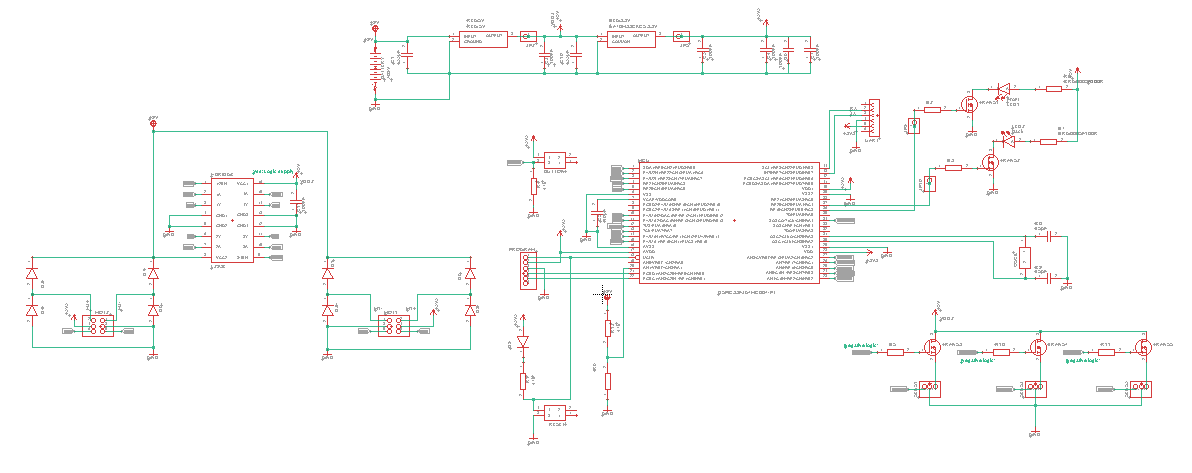
\includegraphics[width=1\textwidth]{figures/hardware/Schematic.PNG}
    \caption{Schematic overview of the micromouse}
    \label{fig:schematic_overview}
\end{figure}

\noindent
This can look intimidating at first and definitely not readable in such a miniature picture. So, let's break it down to its components and describe its sub-circuits. Notice that all of the components appearing in the Schematic were downloaded one by one from the suppliers' site, together with their PCB models, as will be seen later.

With the exception of the first subsection, the components will be presented from left to right and from top to bottom, so that the reader may always refer to the overview schematic to get a clear picture of a component's relation to the whole.

\FloatBarrier
\vspace{1cm}

\subsubsection{Microcontroller (MCU)}

The microcontroller (mcu) can be seen in Fig. \ref{fig:mcuL}.
Notice that the symbolic representation of the mcu, specifically when it comes to the location of its pins, doesn't correspond to the real model. For the purpose of the schematic, we don't really care about the real location of the pins. As will be seen later, this becomes of importance when placing the components on the board to be printed.

\begin{figure}[htb]
    \centering
    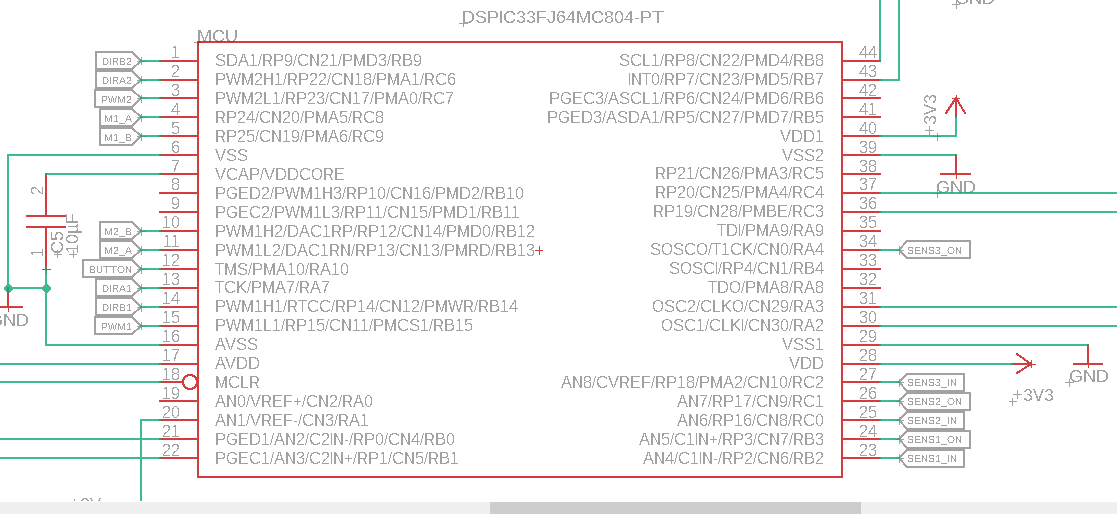
\includegraphics[width=1\textwidth]{figures/hardware/MCU.PNG}
    \caption{The dsPIC33FJ64MC804 microcontroller}
    \label{fig:mcuL}
\end{figure}

\FloatBarrier

\noindent
The assignment of mcu pins to components is presented in the software section and will not be repeated here. Please refer to that section for understanding the functionality of its pins in our circuit.

Another point to notice about the pin connections is the convenient label feature that Autodesk Eagle offers. Notice how some of the components are wired to the pins of the mcu, while other connections are represented as labels. Labels in the circuit are the equivalent of wires and greatly contribute to the readability and modularity of the schematic. As long as two wires anywhere in the circuit share the same label, they are connected.

A last comment has to be made about the pins of the mcu: The pins, as everything in our circuit, are very real components and therefore are subject to electrical limitations. This is a very important point to keep in mind, when driving any load, such as LEDs or a motor, but also when connecting input signals, such as sensors.
Specifically, in the section "Electrical Characteristics" in the mcu datasheet \cite{mcu}, we find maximum values for individual pins and for all utilized pins combined. These can be seen in Fig. \ref{fig:electrical}. These characteristics lead to some important design decisions, specifically named in later subsections.

\begin{figure}[htb]
    \centering
    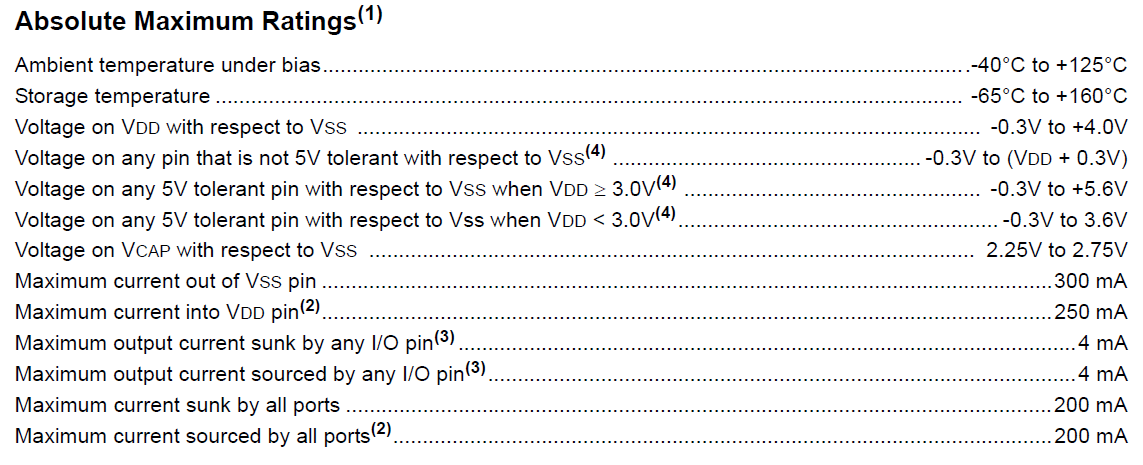
\includegraphics[width=0.8\textwidth]{figures/hardware/Electrical.PNG}
    \caption{Electrical limitations for the pins of the mcu}
    \label{fig:electrical}
\end{figure}

\FloatBarrier
\vspace{1cm}

\subsubsection{Voltage Regulators}

The necessity for voltage regulators, which can be seen in Fig. \ref{fig:battery}, arises from the need for different voltages present in our system. 
Specifically, as found in \cite{mcu}, the mcu considers 3.3V as logical one and it is this voltage we need to provide to it (see $V_{DD}$ pins). The distance sensors used (taken from a previous micromouse model) need 5V. And yet the motors need 6V, as can be seen in \cite{motor}. 
Notice that we are using a battery of 9V. Therefore, we need a way to generate the required three different voltages.

\begin{figure}[htb]
    \centering
    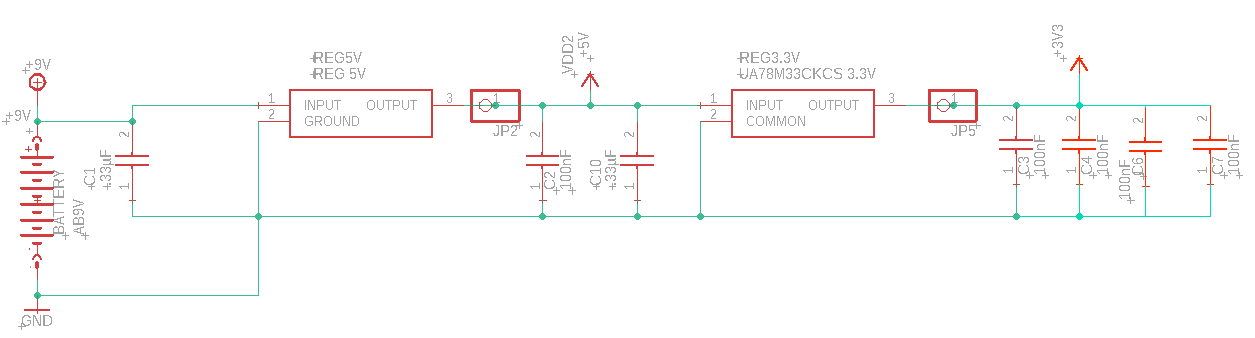
\includegraphics[width=1\textwidth]{figures/hardware/VoltageandCapacitors.PNG}
    \caption{The battery and voltage regulators}
    \label{fig:battery}
\end{figure}

\FloatBarrier

When it comes to the motor, we can regulate the voltage we feed it with, by regulating the maximum duty cycle of the PWM (explained in another section). So, we provide it with a fraction of the available 9V.
For the distance sensors and the mcu, two voltage regulators are used in succession. They provide our components with steady voltage, necessary for functioning properly. A voltage regulator essentially contains a variable resistor, which changes according to current needs of the load, e.g. the mcu, in order to provide a stable voltage in its output.

A question that arises is: Why use 9V, when much less is actually needed in the circuit? One needs to keep in mind that voltage regulators need a minimum difference between the input and the output voltage to ensure steady output voltage. This difference is called "dropout voltage" and can be found in the datasheets of the voltage regulators \cite{3.3V}, \cite{5V}. For example, the dropout voltage of both the regulators we have chosen for our micromouse is 2V. So, one sees that provision for higher extra voltage has to be made.

Now, notice the capacitors used in Fig. \ref{fig:battery}. Capacitors are used in the input and output of the voltage regulators. As can be read in the datasheets of the regulators \cite{3.3V}, \cite{5V}, the capacitors' values are well specified and they are required for the behavior of the regulators to be optimal. Specifically, the input capacitor functions as noise filtering for the voltage supply and the output one ensures improved transient response. For a deeper understanding on the transient response of regulators, refer to \cite{regul}. The article refers to low-dropout linear regulators (it"s not the case for the voltage regulators used here, with 2V dropout), but the main principle of the output capacitor holds just the same.

Additionally,  few capacitors can be observed at the far right part of the sub-circuit.
These capacitors have both a special name and function: They are called decoupling capacitors and their role is to help provide steady voltage and current to the load (here our mcu). Specifically, they are always physically connected close to their corresponding component and should a temporary lack of electrons happen, they provide from their surplus, keeping the voltage and current steady. Such an event can happen frequently, since the mcu is a load that changes its demands on current, depending to the components it's,  in turn, connected to. By changing the demand on current, the voltage regulator, being essentially a variable resistor, needs to readjust, in order to provide the new current. This refers to the transient response of the regulator and it takes a small amount of time for the regulator to adjust. During that time, the decoupling capacitor offers the electrons and thus the current needed.

The decoupling capacitors are only symbolically placed there in the circuit. In reality, they are connected between the pins of the mcu that connect to $V_{DD}$ (3.3V) and ground (GND). Every decoupling capacitor is ideally connected as close to the actual component pins as possible, as will be later seen in the PCB Section. The values of the capacitors are dictated by the datasheets of the specific components used. For example, have a look in \cite{mcu}.

\vspace{1cm}


\subsubsection{H-bridge and Motors}

Next, the motors and H-bridge sub-circuit will be presented. 
First, let us consider the motors. As can be seen in Fig. \ref{fig:motors}, the motors are symmetrically connected to the H-bridge and to the mcu. So, let us concentrate on one of them, the left. The same explanation applies for the other one.

\begin{figure}[htb]
    \centering
    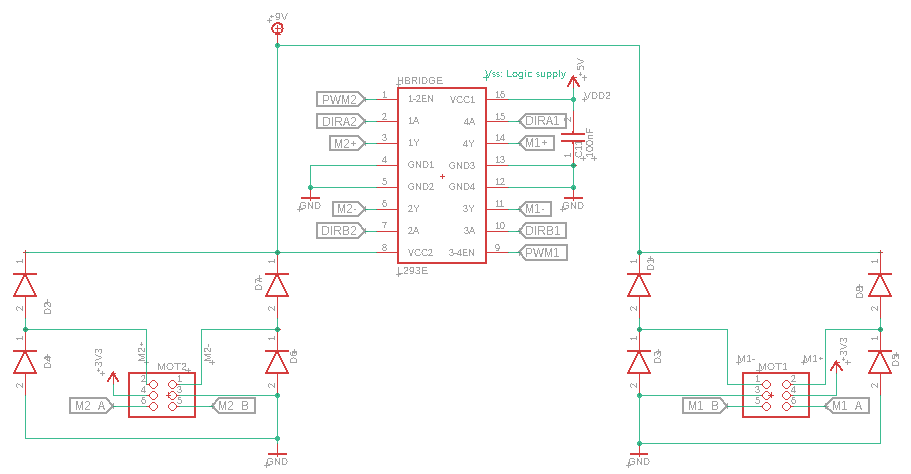
\includegraphics[width=1\textwidth]{figures/hardware/Motors.PNG}
    \caption{The motors and the H-bridge}
    \label{fig:motors}
\end{figure}

\FloatBarrier
\noindent
In Fig. \ref{fig:motorPins} taken from the motor datasheet, the motor pins can be noticed. 
One pair of pins (1, 2) refers to the voltage we feed to the motor. Remember that we are using PWM (max 6V) to control how fast the motor turns and notice that if the voltage is reversed, the rotation of the motor is also reversed. As we will shortly see, for this purpose, the H-bridge is needed. The function of reversing the motor's rotation is highgly desirable, since we want our 2-wheels micromouse to be able to move backwards and to turn on spot (imagine one wheel moving to one direction and the other to the opposite direction with the same velocity).

\begin{figure}[htb]
    \centering
    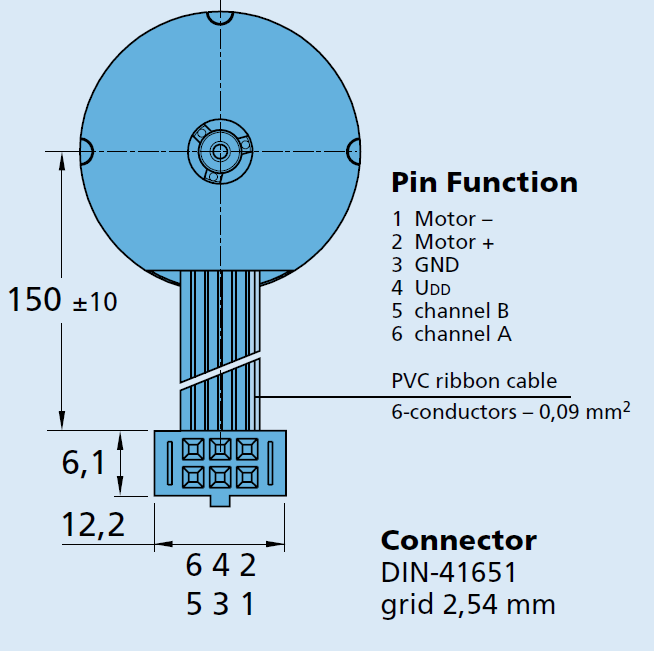
\includegraphics[width=0.8\textwidth]{figures/hardware/motor.PNG}
    \caption{The motor pins as presented in its datasheet}
    \label{fig:motorPins}
\end{figure}

\FloatBarrier
\noindent
Another pair of pins (3, 4) refers to the voltage feed of the motor encoder. And the last pair of pins (5, 6) is used for the output of the motor encoder signals. These signals encode the motor's rotational position every moment and are fed to the mcu. In the mcu, with the help of the quadrature encoder (QE) module, they can be translated to real position in space.

Finally, let us consider the H-bridge. As mentioned, the need for the H-bridge arises from the function of reversing the motor polarity and thus its rotation. Without the use of an H-bridge, one would have to physically reverse the wires for the motor feed. If it is impractical with the use of wires, it is impossible with the traces on a PCB. Instead, the H-bridge can conveniently reverse the voltage. 

The main principle of an H-bridge can be seen in Fig. \ref{fig:HPrinciple}. The bridge functions with a pair of switches (MOSFETs in the figure). When one pair is closed, current flows through the motor and it rotates to one direction. Notice that at the same time, the other set of switches is open. When we want the motor to rotate in the other direction, the other set of switches closes and this one opens. A time delay is necessary, when all switches are open, else the voltage source will be short-circuited and this is something we want to avoid at all costs.

\begin{figure}[htb]
    \centering
    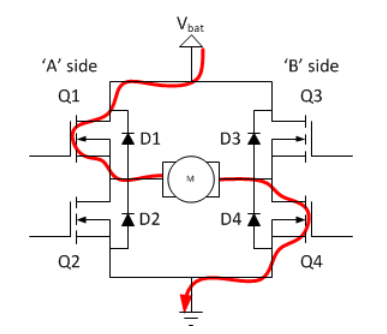
\includegraphics[width=0.8\textwidth]{figures/hardware/H-Principle.PNG}
    \caption{The principle of how an H-bridge allows flipping rotation direction of the motor, taken from \cite{catchDiodes}}
    \label{fig:HPrinciple}
\end{figure}

\noindent
Next, have a look at the exemplary circuit in Fig. \ref{fig:HData}, taken from the datasheet of the H-bridge \cite{Hbridge}.

\begin{figure}[htb]
    \centering
    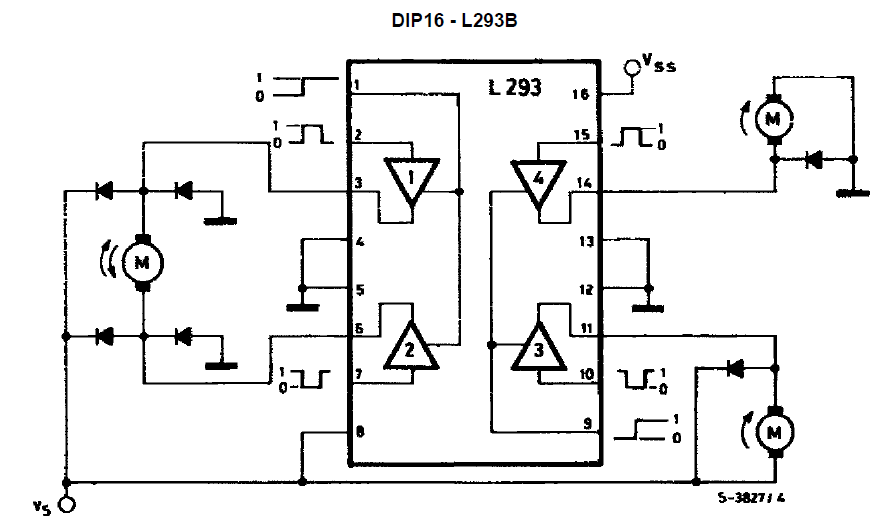
\includegraphics[width=0.8\textwidth]{figures/hardware/HbridgeDatasheet.PNG}
    \caption{Exemplary motor connection from the H-bridge datasheet}
    \label{fig:HData}
\end{figure}

\FloatBarrier
\noindent
We feed our PWM in pin 1. Pins 2 and 7 are used for controlling the direction of rotation of the motor. The truth table is simple: If one direction pin is "1" and the other "0", then the logical "1" defines the direction. If both of the pins are set to logical "0" or "1", the motor breaks. Notice how the pins 3 and 6 feed the voltage to the motor and are coupled with the direction pins. Comparing figures \ref{fig:HPrinciple} and \ref{fig:HData}, the direction pins in the latter hide inside them the functioning pair of switches mentioned in the earlier.

As a last comment, in both Fig. \ref{fig:HData} and Fig. \ref{fig:motors} notice the existence of diodes. Again, these diodes have both a special name and a special function. They are called \textit{catch diodes} and to understand their use, please refer to \cite{catchDiodes}, where a beginners-friendly introduction to H-bridges is offered.
For our purposes, it suffices to say that the presence of catch diodes is necessary for the smooth functioning of our brushed motor. Consider the case, when the motor changes direction or stops from spinning. In order for this to happen, the internal switches of the H-bridge need to open (remember the direction pins). Temporarily, the current that was flowing in the circuit through the motor has to go ("escape") somewhere, since due to the inductance nature of the motor, the current cannot instantly go to zero . It is not a good idea to dissipate the current through our H-bridge pins/ switches, without an alternative: The current will try to jump an open switch, creating a spark and probably burning the pin/switch. The catch diodes provide this alternative: The current flows through them in a forward way and is returned to the source.

\vspace{1cm}


\subsubsection{Extra Button}

Naturally, the more input options we have for our micromouse robot, the more flexible the commands we can issue and the more complicated the software can be. Therefore, we added a button (switch), which can be seen in Fig. \ref{fig:button}.

\begin{figure}[htb]
    \centering
    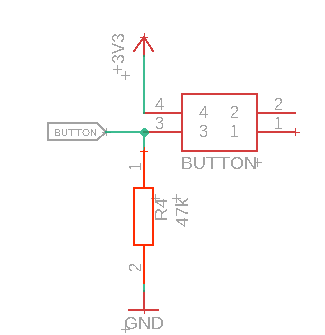
\includegraphics[width=0.8\textwidth]{figures/hardware/Button.PNG}
    \caption{An extra button for input}
    \label{fig:button}
\end{figure}

\FloatBarrier
\noindent
A typical pull-down resistor of 47k is used, to make sure the mcu pin never has an undefined logical value ("floating"). When it comes to the resistance value, it is somewhat arbitrary in that it does its job. A different value could have been selected.
For the current that flows through the resistor, when the button is pressed, we have:

$$V = I*R => 3.3 = I*47 => I = 0.07mA$$

If a much smaller value for the resistance was used, then the current would be much larger, leading to unnecessary power dissipation on the resistance and heating. Also, in this case, there is the possibility for the input to the mcu pin to be stuck in a low, logical 0 level, no matter if the button is pressed or not.

\vspace{1cm}


\subsubsection{Programmer}

The programmer is the device that allows for (re)programming of the mcu. The way it is connected is rather straightforward and can be seen in Fig. \ref{fig:programmer}.
Of particular interest is the use of the MCLR pin (Master Clear) in the mcu. In order for the EEPROM (electrically erasable programmable read-only memory) to be reprogrammed, the programmer device needs to raise the voltage of this pin higher than $V_{DD}$. The MCLR pin is used both for programming and resetting purposes.

\begin{figure}[htb]
    \centering
    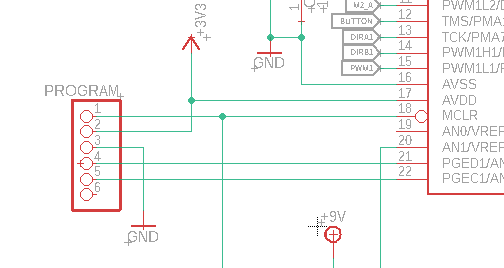
\includegraphics[width=0.8\textwidth]{figures/hardware/Programmer.PNG}
    \caption{The programmer}
    \label{fig:programmer}
\end{figure}

\noindent
More details about the reprogramming of the flash memory of the mcu can be found in \cite{mcu}, in the section "FLASH PROGRAM MEMORY".

\FloatBarrier
\vspace{1cm}


\subsubsection{Reset Button}

A reset button is needed in case something goes wrong during the execution of the program in the mcu, or if one simply needs to start the execution from the start again. Notice that the MCLR (Master Clear) pin is also used by the programmer for programming and debugging, as can be found in \cite{mcu}.

\noindent
The reset activation logic in our mcu is negative or inverse, as can be seen in Fig. \ref{fig:reset}. A diode and a pull-up resistor (similar to the pull-down used for the other button) connect the voltage feed to the mcu. Once the button is pressed, a connection with the ground is made and the mcu is reset. Remember from the previous section, that during programming of the mcu, the voltage for this particular pin is raised higher than 3.3V. For this reason, the diode is needed in series with the pull-up resistor.
Again the choice of the resistance value is a bit arbitrary.

\begin{figure}[H]
    \centering
    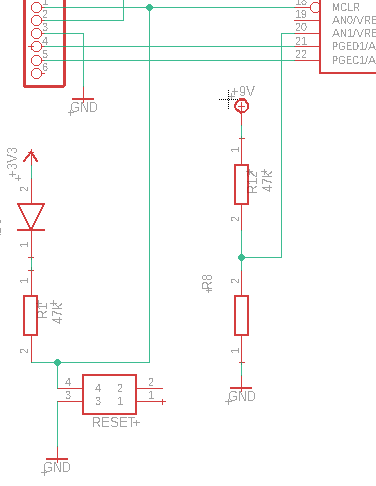
\includegraphics[width=0.8\textwidth]{figures/hardware/MCLRandBatteryMeasurement.PNG}
    \caption{The reset button and the battery voltage measurement circuit}
    \label{fig:reset}
\end{figure}

\vspace{1cm}


\subsubsection{Battery Measurement}

In an ideal world, our battery would provide steadily 9V until its exhaustion. However, this is not the case. As the battery is depleted, the voltage it provides is reduced. It would be useful to know exactly how much voltage the battery provides at any given point in time. Feeding this value to the mcu, we can take decisions accordingly. For example, we can regulate the PWM maximum duty cycle value to keep the motor spinning at its maximum velocity, even though the battery is depleted. Remember that our motor can take a maximum of 6V for its fastest performance.

Additionally, as described in the subsection \textit{Voltage Regulators} above, the voltage regulators have a characteristic dropout voltage. In this case, the 5V voltage regulator will stop providing steady 5V, once the battery starts offering less than 7V. This means, that our circuit will malfunction, from the mcu to the distance sensors. We need to detect this in time to change the battery.

In order to realize such a schema, a simple voltage divider sub-circuit and an analog pin of the mcu can be used, as can be seen in the above Fig. \ref{fig:reset}.
In order to keep the amount of different components to a minimum, a resistance of 47k is used. The question now is, what should the value of the other resistance be, in order for the input voltage to the mcu to be 3.3V for a 9V battery. 

If we call the unknown resistor $R_8$, as in the figure, we can use the known equation for a voltage divider:

$$V_{MCU} = \frac{R_8}{47+R_8} * 9V = 3.3V$$

\noindent
With a value of $ R_8 = 22k $, we can easily calculate the resulting $V_{MCU} = 2.87V$. This is a convenient value, since for example another battery of higher voltage, e.g. 10V, could be used. By choosing this value we fulfill our initial purpose and have some flexibility for higher voltages.

\FloatBarrier
\vspace{1cm}

\subsubsection{Universal Asynchronous Communication (UART)}

Despite us building an autonomous micromouse robot that can navigate in a labyrinth, we would still like to be able to issue stand-alone commands via UART. Hence, the UART sub-circuit of Fig. \ref{fig:uart}. The connection is straight-forward. Only attention is required in connecting RX to TX of the mcu and vice-versa.

\begin{figure}[htb]
    \centering
    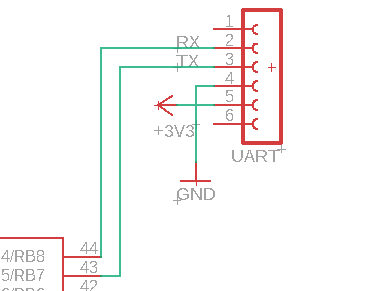
\includegraphics[width=0.8\textwidth]{figures/hardware/UART.PNG}
    \caption{The UART module}
    \label{fig:uart}
\end{figure}

\FloatBarrier
\vspace{1cm}


\subsubsection{Light-emmiting Diodes (LEDs)}

To motivate the use of two LEDs in our micromouse, imagine the following: The PCB lies on the two wheels, which are screwed on either side somewhere in the middle. Naturally, the PCB will tilt forwards or backwards until it touches the ground, depending on where most weight lies (front sensors). This is highly unwanted: Not only would it result in an unelegant movement creating uneccessary impedance, but the PCB could be potentially damaged by friction and by ground anomalies.

Therefore, for mechanical stability, we use one LED on the front and one on the back of our PCB. They are through-hole components, with the head of the LED resting on the under side of the PCB. The smooth surface of the head works to our favor, not only stabilizing the micromouse, but also offering minimum resistance while moving. The height of the protruding LED head can be decided during soldering according to mechanical needs.

Now, since we have the LEDs, it would be nice to be able to turn them on and off at will. For example we can light the front LED when the micromouse is moving forward and the back one when it's moving backwards.
The sub-circuit for controlling the LEDs can be seen in Fig. \ref{fig:leds}.

\begin{figure}[htb]
    \centering
    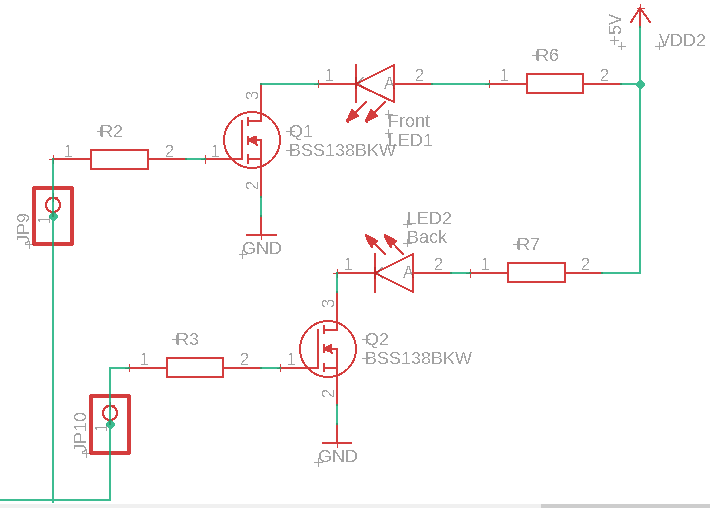
\includegraphics[width=0.8\textwidth]{figures/hardware/LEDs.PNG}
    \caption{The LEDs used for mechanical stability}
    \label{fig:leds}
\end{figure}

\FloatBarrier
\noindent
The sub-circuits for both LEDs are identical, so let us examine one of them, say the front one. The main component, besides the LED, is an N-channel metal-oxide semiconductor field-effect transistor (MOSFET).

To motivate the need for the MOSFET, imagine connecting the LED directly to the I/O pin. In the datasheet of a typical low current LED (and also the one we will be using) \cite{leds}, we find that the current can be somewhere between 25 to 140 mA. However, the value of 140mA can only be reached under certain PWM conditions. In our case, 20mA steady current will suffice for a bright enough LED. Also the voltage drop on the LED is 2.2 to 2.5V for $I = 20mA$.

Remember the electrical characteristics of the mcu pins as presented in Fig. \ref{fig:electrical}. Notice that the limit current per pin is 4mA! In other words, if we directly connect the LED to the mcu, we will damage the mcu pin and potentially other parts of the mcu circuit. 
Now, the MOSFET serves as a switch: By providing a low current to its gate (the pin of the MOSFET connected to the mcu pin), its channel between the drain and source opens. In other words, it allows current to flow from the LED side to the ground side, thus closing the circuit and lighting the LED up! 

The resistor R2 in the sub-circuit is used to charge the capacitance of the transistor gate. Hence its value is not critical in our case, since no intense time precision demands are made on the LED. We can use our typical 47k resistors also here. Notice that exactly next to the mcu pin, a header pin is placed with the name JP9. This is just a convenient way to later check the voltage of the pin on the PCB for debugging purposes.


The last component to cover is the resistor on the side of the LED. To choose an appropriate value, we need to consider the voltage drop on the LED. As we read above it's somewhere between 2.2 and 2.5V. We can use $\Omega$hm's law, by considering the resistance of the transistor negligible and the resistance of the diode fixed. For the current flowing, let's choose 20mA as stated above. 

$$V_R = I * R => 5 - V_{diode} = I * R$$

For the values $V_{diode} = 2.2V$ and $I = 20mA$ we acquire a value of 140$\Omega$. So, this is the value we need for the resistor.

\vspace{1cm}

\subsubsection{Oscillator}

The external oscillator and its capacitors can be seen in Fig. \ref{fig:oscillator}. As can be found in the datasheet of the mcu \cite{mcu}, the internal oscillator offers up to 8MHz frequency. For this reason and also for the flexibility of being able to choose, we opted out for a 16Mhz external oscillator.
The capacitors are necessary for the functioning of the crystal oscillator, since they are not included in it.

\begin{figure}[htb]
    \centering
    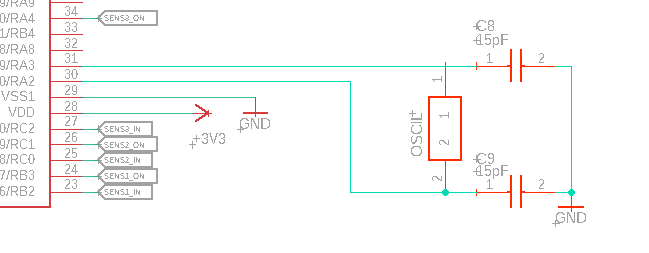
\includegraphics[width=0.8\textwidth]{figures/hardware/Oscillator.PNG}
    \caption{The external oscillator}
    \label{fig:oscillator}
\end{figure}

\FloatBarrier
\vspace{1cm}


\subsubsection{Distance Sensors}

The distance sensors are necessary for perceiving the distance from maze walls. Their sub-circuit can be seen in Fig. \ref{fig:sensors}.

\begin{figure}[htb]
    \centering
    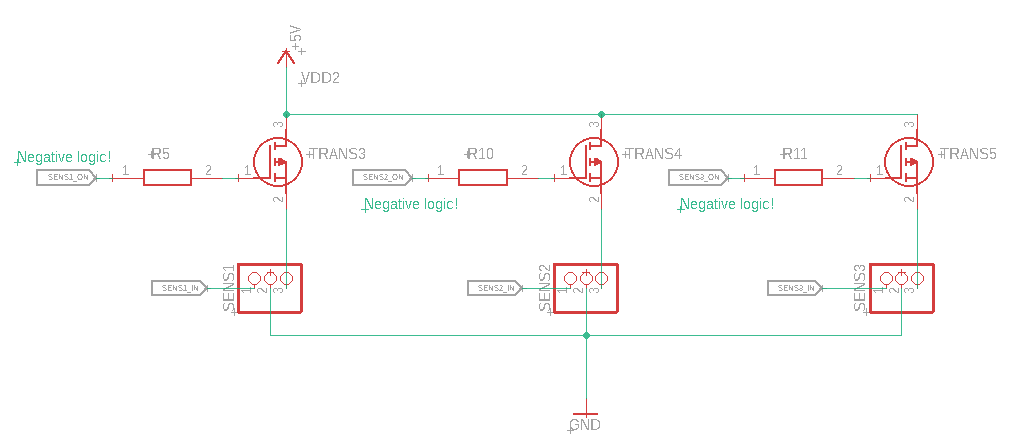
\includegraphics[width=1\textwidth]{figures/hardware/DistanceSensors.PNG}
    \caption{The distance sensors}
    \label{fig:sensors}
\end{figure}

\FloatBarrier

To understand their pins, have a look at Fig. \ref{fig:sensorsData} taken from the datasheet \cite{sens}.

\begin{figure}[htb]
    \centering
    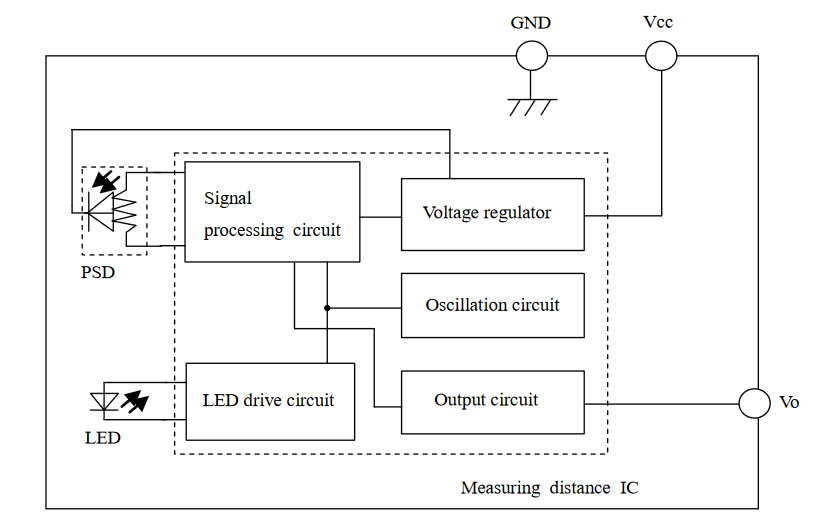
\includegraphics[width=0.8\textwidth]{figures/hardware/sensorData.PNG}
    \caption{Internal schematic of the distance sensors}
    \label{fig:sensorsData}
\end{figure}

\FloatBarrier

\noindent
Instead of connecting the voltage feed directly to 5V, we use a P-channel MOSFET to turn the sensors on and off at will. The connection of the transistor is the opposite of the N-channel described above (Section LEDs) and its functionality is the same: It is used as a switch. Notice the 47k resistors that connect the gates of the transistors to the pins of the mcu. By offering current from the pins, we close the switch and activate the sensors. Being able to turn the sensors on and off mostly offers flexibility in software.

Last, we feed the incoming data from the sensors to dedicated analog pins in our mcu.

\vspace{1cm}


\subsection{Components}

In this section, we list the actual components we chose to order. Most of the components were ordered from \textit{RSComponents}, Fig. \ref{fig:compRS} and the rest from \textit{Mouser}, Fig. \ref{fig:compMou}. The purpose of the lists provided are simply for reference. The components chosen are not a unique solution. Also, the choice of supplier was mostly made due to component availability reasons.

\begin{figure}[htb]
    \centering
    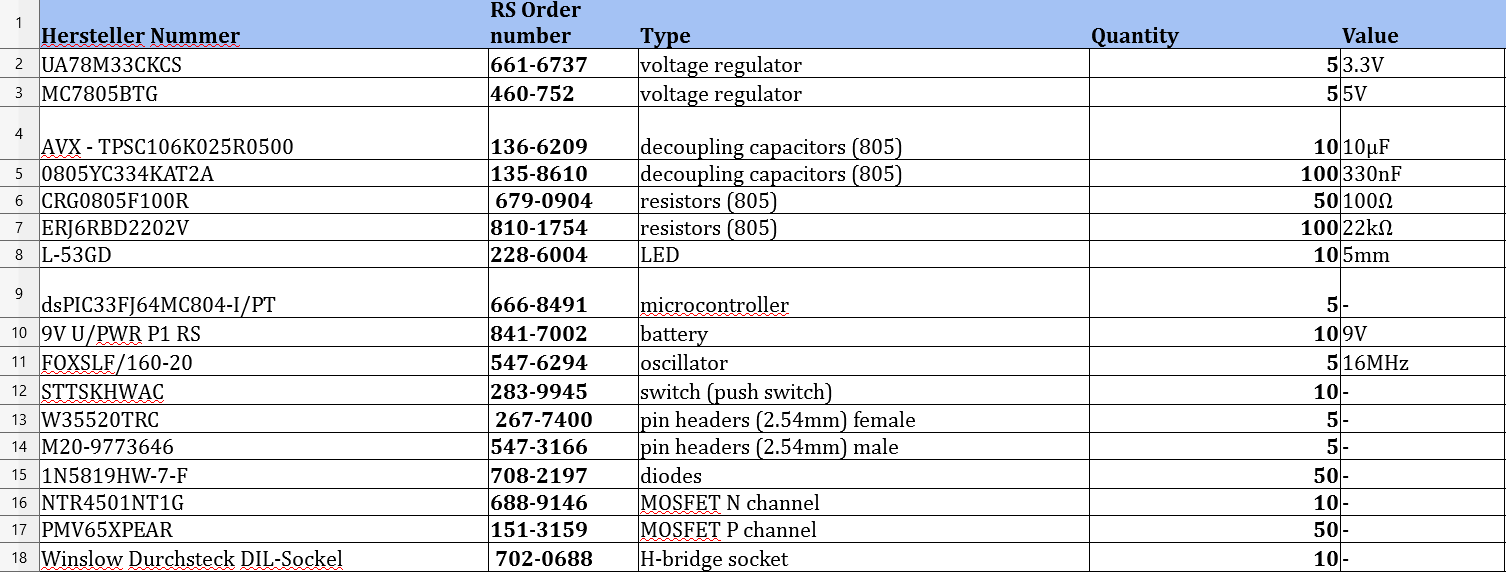
\includegraphics[width=1\textwidth]{figures/hardware/Components1.PNG}
    \caption{Components ordered from RSComponents}
    \label{fig:compRS}
\end{figure}


\begin{figure}[htb]
    \centering
    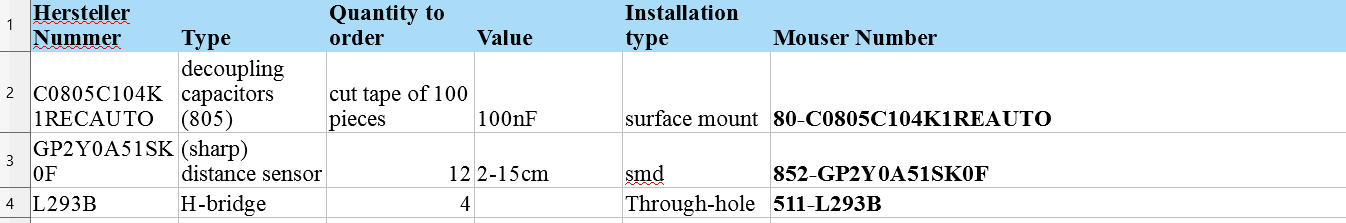
\includegraphics[width=1\textwidth]{figures/hardware/Components2.PNG}
    \caption{Components ordered from Mouser}
    \label{fig:compMou}
\end{figure}

\FloatBarrier
\noindent
Notice that the quantities mentioned are not referring to one board only. The quantities ordered were chosen with the thought of building four PCBs, checking the availability of existing components in the lab and the minimum components order of the suppliers. 
For the number of components needed per board, please refer to the Schematic and Fig. \ref{fig:comp1} and \ref{fig:comp2}.

\begin{figure}[htb]
    \centering
    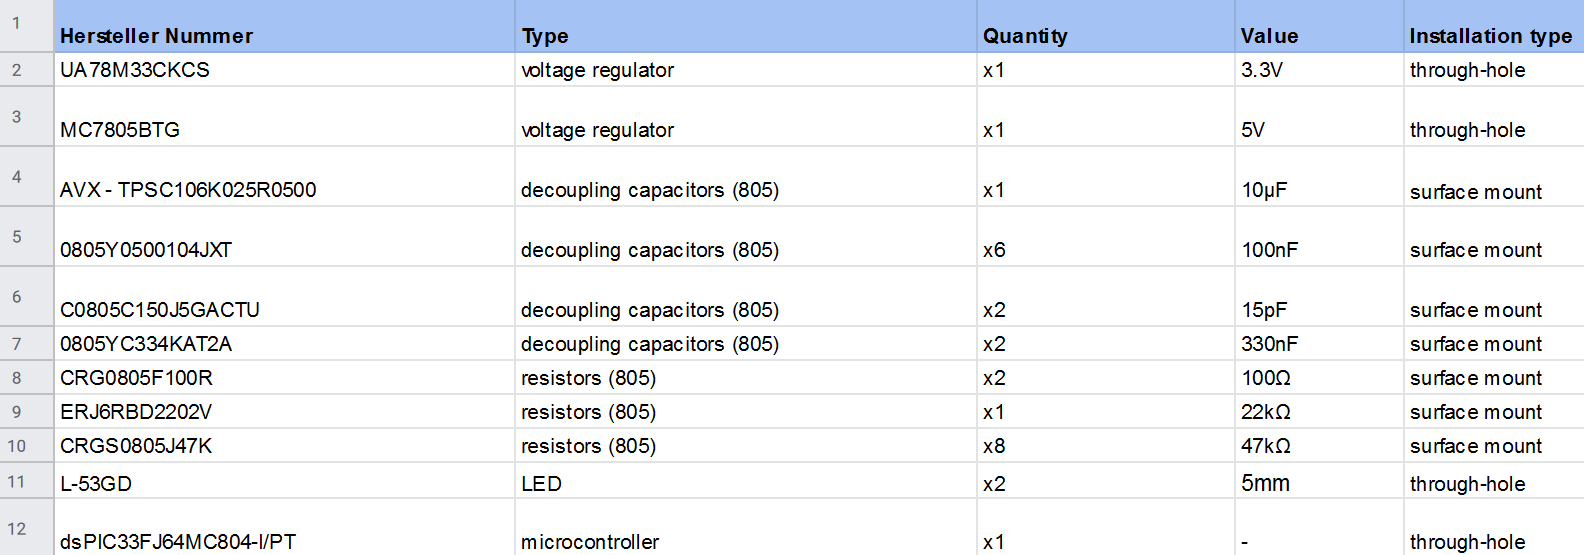
\includegraphics[width=1\textwidth]{figures/hardware/CompList.PNG}
    \caption{List of components needed for one PCB}
    \label{fig:comp1}
\end{figure}


\begin{figure}[htb]
    \centering
    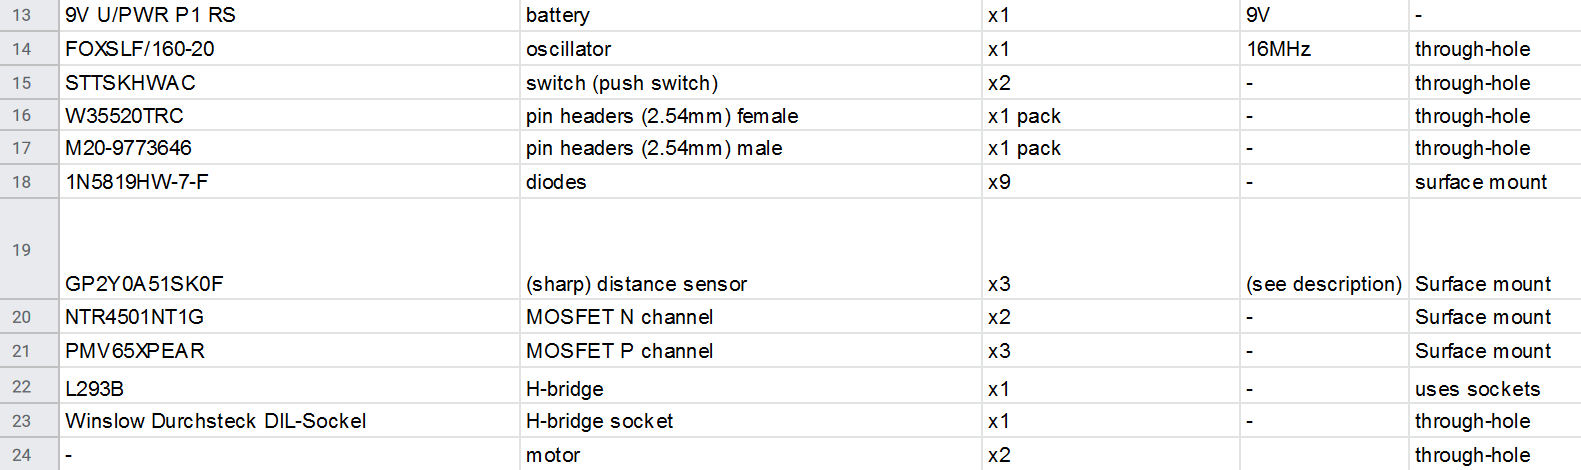
\includegraphics[width=1\textwidth]{figures/hardware/CompList2.PNG}
    \caption{List of components needed for one PCB (cont.)}
    \label{fig:comp2}
\end{figure}
\FloatBarrier

\vspace{1cm}


\subsection{Printed Circuit Board (PCB)}

In this Section, the PCB of the micromouse will be presented. All in all, the PCB is the body and soul of the robot: Its physical aspect constitutes the largest part of the robot, hosts the mcu (the brain of the robot) and all the necessary components already described in the Schematic Section. 
The finished PCB can be seen in Fig. \ref{fig:pcb}. The dimensions are: From head to tail 11.6 cm and from side to side 8.5 cm. The printed PCB can be seen in Fig. \ref{fig:print} .

\begin{figure}[H]
    \centering
    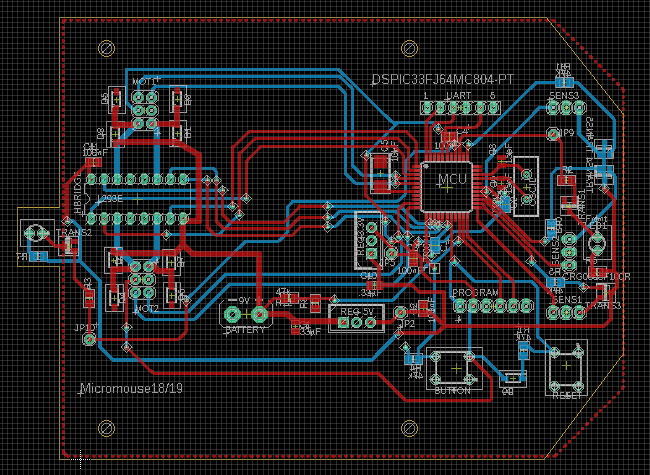
\includegraphics[width=0.8\textwidth]{figures/hardware/PCB.PNG}
    \caption{The final PCB version}
    \label{fig:pcb}
\end{figure}

\begin{figure}[H]
    \centering
    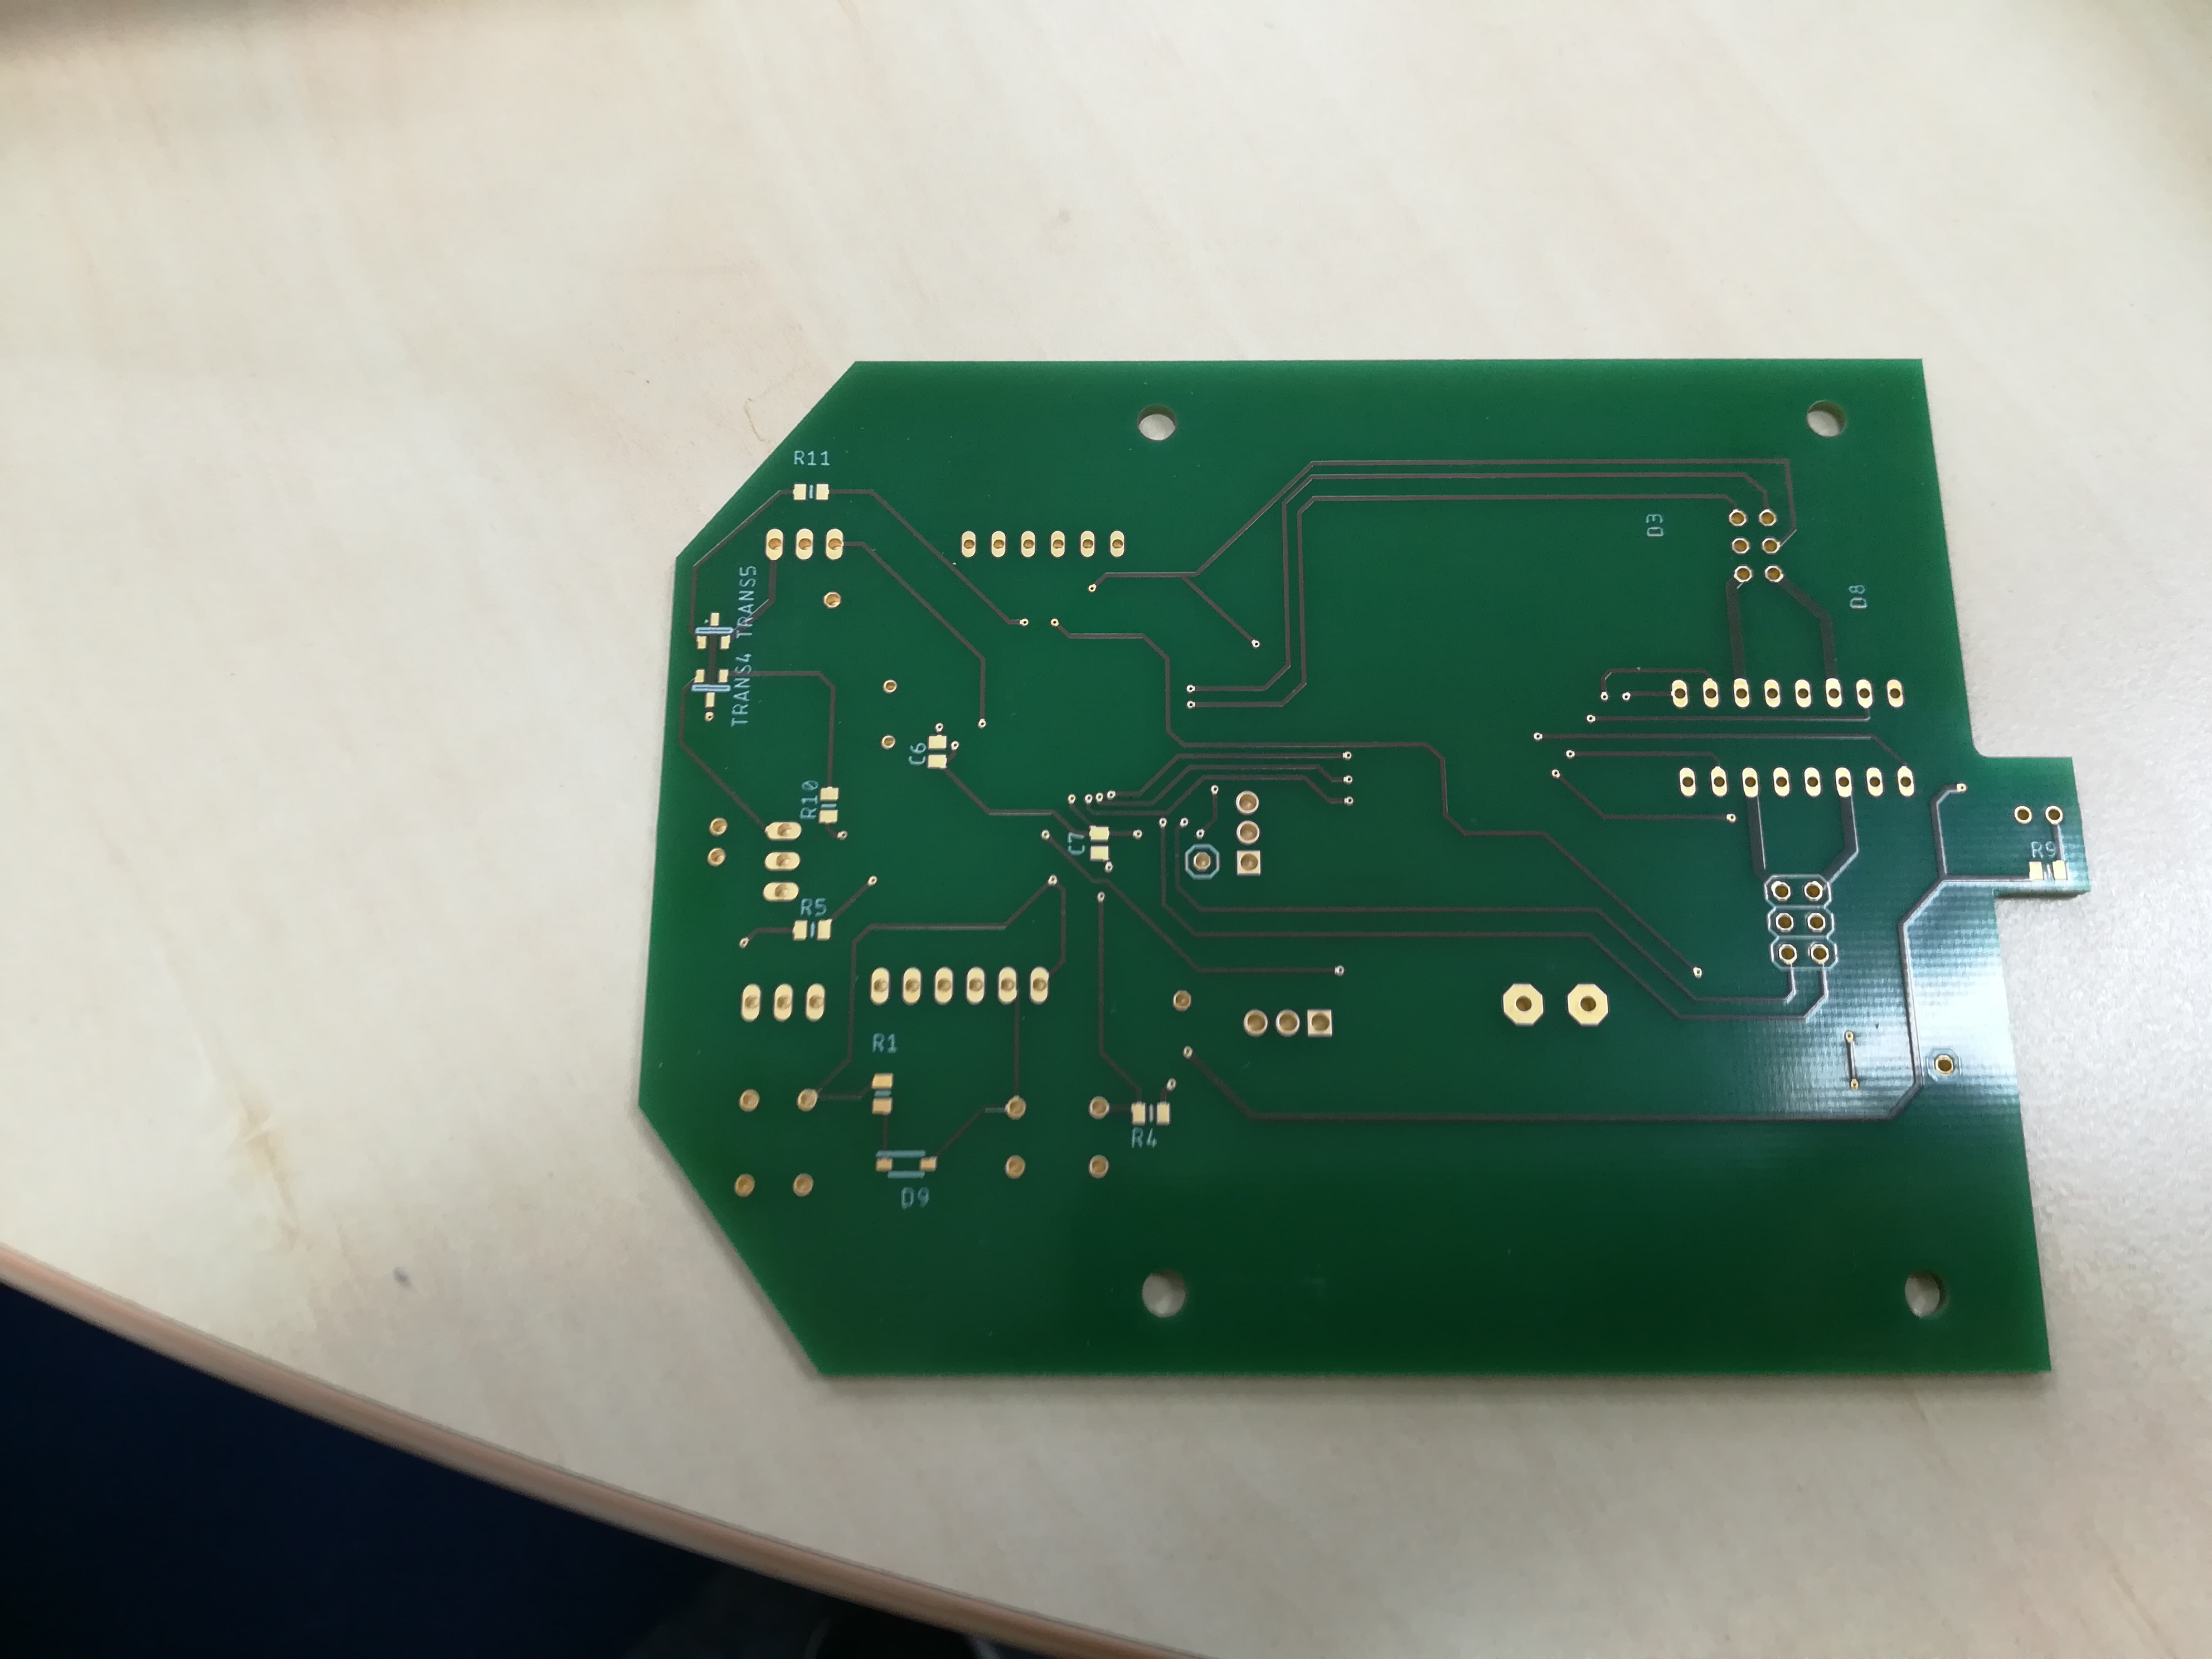
\includegraphics[width=0.8\textwidth]{figures/hardware/printed.jpg}
    \caption{The printed board (bottom layer)}
    \label{fig:print}
\end{figure}

\noindent
Our PCB features two layers: The top and bottom layer. Keep in mind that they are both physically and electrically isolated, unless we deliberately create a connection, as explained later. All necessary concepts are explained when needed in the following subsections, so it is important to read through them in order.\\
The process roughly consists of three steps, corresponding to the subsections that follow.

\FloatBarrier

\subsubsection{Components Placing}

Generating the PCB board from the Schematic is straight-forward in Eagle: The software offers an empty board and the models of the Schematic components placed out of it.

The first step of the procedure is to actually place the components on the board. There are no hard restrictions here, but rather a few rules of thumb. For example, it is desirable to reduce the size of the PCB as much as possible, but still place the components comfortably enough for connections to be made (traces). So a good trade-off has to be found. Before we continue with more examples of such rules, there are few details that need to be mentioned.

It is important to notice here, that the casing of the components was chosen as 805 and not smaller. We wanted a size that would allow us to comfortably solder the components on the board.

The final placement of components can be seen in Fig. \ref{fig:comp}.

\begin{figure}[htb]
    \centering
    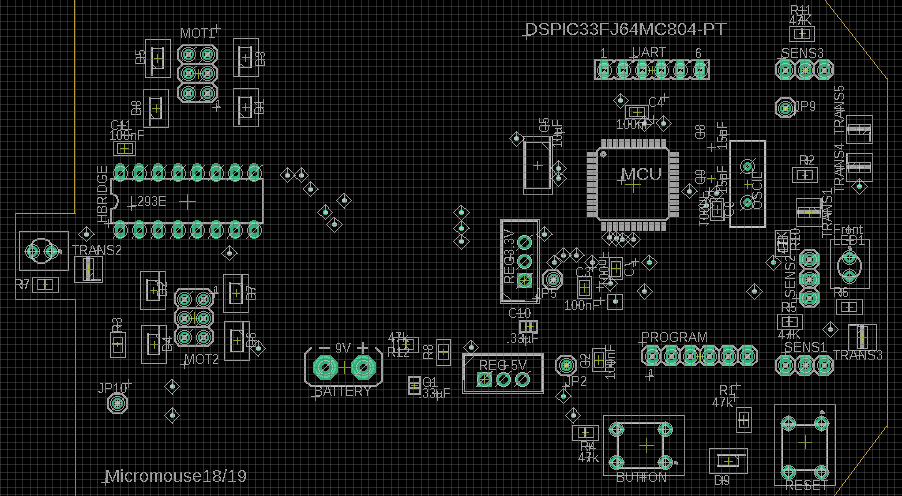
\includegraphics[width=0.8\textwidth]{figures/hardware/PCB_Components.PNG}
    \caption{The final placement of components on the PCB}
    \label{fig:comp}
\end{figure}

As mentioned, in our case, a two layer PCB is designed. The top and bottom layers, both contain components. To fully appreciate this fact, notice that there are two different kinds of components used on a PCB: Through-hole and surface mount (SMD). 

The through-hole components actually go through the PCB. The manufacturer needs to drill holes for this purpose. An advantage of this type is mechanical stability. Another advantage comes in the tracing phase, when connecting the components: The through-hole ones can have traces leading to and from them in both the top and bottom layers. The reason is obvious, they have physical presence in both layers, since they go through the surface of the PCB to the other side. However, the whole concept does occupy more space than the SMD components. Also, drilling holes costs more, when ordering the PCB.

Now the SMD components are soldered only on the surface of the PCB (top or bottom layer) and no drilling is required. They occupy less space too. However, a track can lead to or from them only in the layer they are found. If a connection between SMD components in different layers needs to be made, a change of layer on the track is necessary, somewhere in its course. We will come back to tracing in the next subsection. 

\FloatBarrier
\vspace{1cm}

For now, let us consider some of the needs that led to this particular placement of components. The following train of thought is definitely not unique and a different placement could have been chosen.

Referring to Fig. \ref{fig:comp}, let's start with the sensors' pin headers. It is clear that the distance sensors need to  be placed in the front (right side of the PCB). Therefore their pins have to be placed nearby. Now, notice the analog nature of the sensors output: We want the traces of those signals to the mcu to be as short as possible, since analog signals are susceptible to noise. Hence the mcu is placed in the front of the board, as well.

After this choice is done, the location of several components is obvious: The oscillator needs to be as close as possible as well. The decoupling capacitors, whether on the top or bottom layer, need to be placed as close to their connecting pins, as possible. It is a good idea to also place the programmer and the UART pin headers close to the mcu for convenience.

The buttons need not necessarily be placed close to  the mcu. Admittedly, a more convenient location for them could be found on the board, for example one in the front and one in the back.

Notice the empty space in the middle of the board. It is planned for the battery. In our case, instead of using a through-hole battery case on the board, the battery is to be floating above it, in a dedicated case of the casing. Even though it would be possible to dismiss the space kept on the board, we chose to keep it as a plan B, just in case the casing is not available. To the left and right of the battery more space is kept for the motors, dictated by their dimensions and the casing to host them. Finally, notice the four drills at the left and right sides of the board. As will be explained later, the design of the casing allows for sliding the board in it, before the motors and wheels are placed. However, just in case extra stability is needed, these four holes allow for screws to hold the PCB and the casing together.

Since we are still in the middle of the board, notice the two voltage regulators, in succession of the battery pins. It is convenient, in our case, to have the source in the middle of the board.

Moving on to the back of the PCB, the H-bridge needs to be placed in the middle of the two motors' pins. The back LED, much like the front one in placed approximately in the middle of the edge, since its role is mechanical stability. The little tail, where the LED is placed, is just a nice artistic touch, as are the front cuts on the board.


\subsubsection{Tracing (Connecting Components)}

Now that the components have been placed and the shape of the PCB decided, they need to be connected. This procedure is called "tracing", since the components are connected through copper traces on the board.
As mentioned above, the traces can be on the top or bottom layer and the two layers are isolated, hence the traces on different layers are also isolated from each other. 
The final tracing can be seen in Fig. \ref{fig:pcb} above.
A view with the traces on the top layer can be seen in Fig. \ref{fig:top}. The view featuring only the traces on the bottom layer can be seen in Fig. \ref{fig:bottom}.

\begin{figure}[htb]
    \centering
    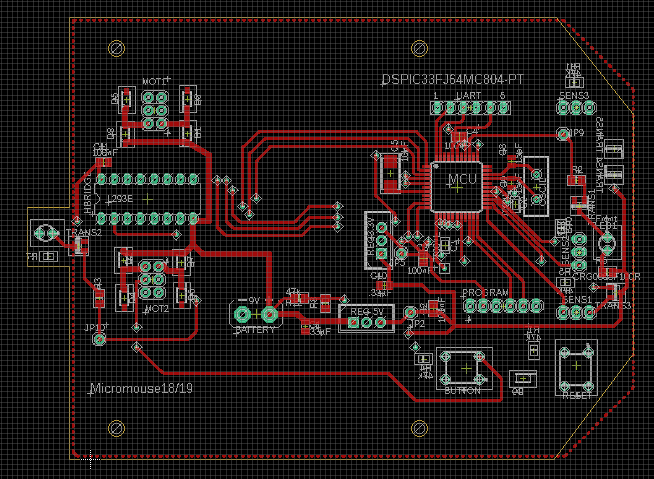
\includegraphics[width=0.8\textwidth]{figures/hardware/PCB_Top.PNG}
    \caption{The PCB with only top layer traces visible}
    \label{fig:top}
\end{figure}

\begin{figure}[htb]
    \centering
    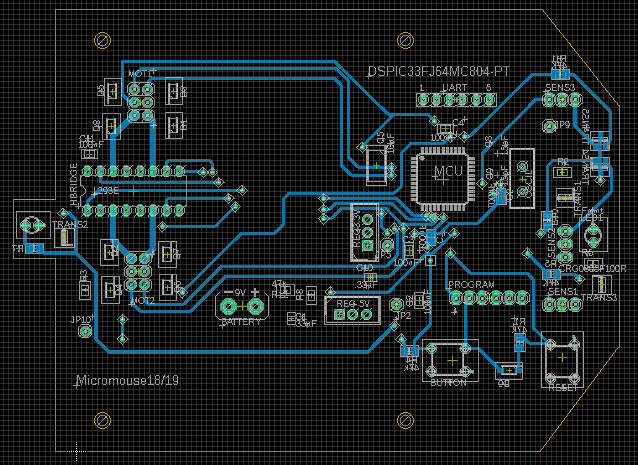
\includegraphics[width=0.8\textwidth]{figures/hardware/PCB_Bottom.PNG}
    \caption{The PCB with only bottom layer traces visible}
    \label{fig:bottom}
\end{figure}

\FloatBarrier
\noindent
This is a good point to introduce the concept of "via points". Notice how traces on the top layer (red) change to traces on the bottom layer (blue) and vice versa. The point where the layer (and color) changes is a via point. A via point is a drill on the PCB, to allow for the trace to change layer. 
Hopefully, the above discussion about SMD and through-hole components makes more sense now. Notice how, in some cases, the traces change layer just before connecting to an SMD component, in order to get to the component's layer.
All in all, drawing traces in an organized manner is not straight-forward. Two restrictions to keep in mind: Keep both the number of via points and the length of the traces as low as possible. The reason for the first being the cost and complexity of the PCB and for the latter, the cost and the accuracy of the corresponding signal: The longer the trace, the larger its resistance, the bigger the noise that is picked up.

One important aspect of tracing is the choice of trace width. So to speak, professionals quickly develop a feeling for this, but for the rest of us, there is always the scientific way:

The total resistance of a trace is given by the following formula

$$R = \rho * \frac{l}{A}$$

Here, $\rho$ is the specific electrical resistance of copper (as material). It equals to $1.68*10^{-8} \Omega *m$ at $20 \degree C$.
l is the length of the trace and A is the height of the trace (usually 0.035mm) multiplied with the width.
In order for the right width to be chosen, we need to consider the desirable value for the resistance. And in order to do that, again $\Omega$hm's Law has to be considered, referring to the current we expect to run through our trace.
This analysis leads to the intuitive result: When we expect a large value for the current, then a smaller resistance is needed and thus a larger width value for the trace needs to be selected. For smaller values of current, smaller width may be selected. In any case, a minimum width is dictated by the manufacturer rules and the good connection of a component's pin.

For example, it is known that motors can draw a lot of current, especially when they first start moving. Thus, the traces to the motors and the H-Bridge need to have a wider width.

Eagle offers a nice feature when it comes to measuring trace length and acquiring an estimation of relevant values. A ULP script provides us with this info, by running the command \textit{run length-freq-ri} in Eagle's command line. An example from our circuit can be seen in Fig. \ref{fig:length}. Notice how the estimation for the maximum current on the trace is shown in the end right column and how the wider traces of the motor (e.g. M1+, M2+, etc.) can take more than 1A.

\begin{figure}[H]
    \centering
    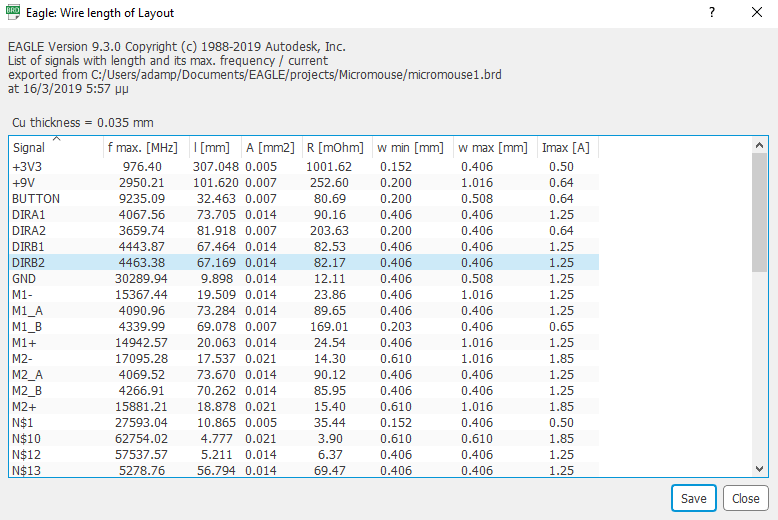
\includegraphics[width=1\textwidth]{figures/hardware/ULP.PNG}
    \caption{Trace length and other info}
    \label{fig:length}
\end{figure}

\noindent
All in all, we kept it simple and well in the limits with  the choice of the width: There are only three different widths in our PCB traces. The largest is 1.016 mm and is used for the connections between the motors, the H-bridge and the battery. Then we have 0.6096 mm for the connections from the 5V regulator (essentially the sensors). Last, the smaller width is 0.4064 mm and is used for all the rest. Especially in the case of the close to each other mcu pins, a larger width would be a nuisance, since there needs to be a minimum clearance between the traces.

\vspace{1cm}

The last concept to be introduced in this chapter is the "ground plane" (GND). The ground plane is a convenient way of connecting all the GND nodes (pins) of the components, meaning the pins that need to be connected to 0V. For our purposes here, we will call it ground. In essence, it is a layer that can be placed on a PCB layer, which connects everything on it. It can be seen in Fig. \ref{fig:gnd}.
In reality, there is a much more important motivation to create a GND plane, instead of connecting pins of components like with positive voltage: Noise rejection. We will not go into this here, but it is worth considering the noise signals coming out of the pcb and the ones produced from the pcb. Closed traces of high-frequency current may function as antennas, when the space they encompass is large. This would be the case if one used traces also for the 0V connections. By using a GND plane, however, this area is kept to a minimum, limiting the noise produced.

\begin{figure}[htb]
    \centering
    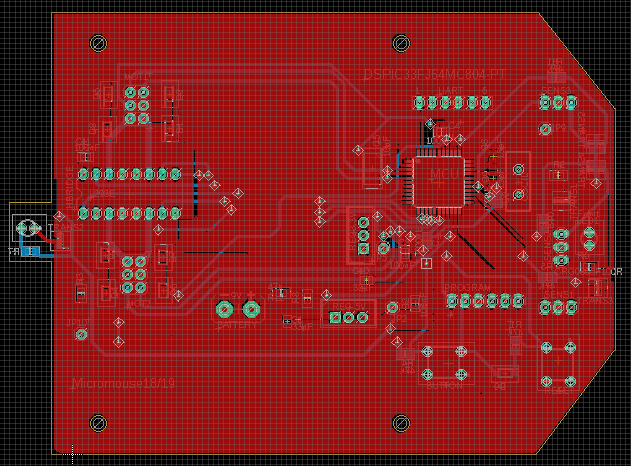
\includegraphics[width=0.8\textwidth]{figures/hardware/PCB_Grounded.PNG}
    \caption{The PCB with the ground plane visible}
    \label{fig:gnd}
\end{figure}

\noindent
The copper traces run through this all-connecting surface, in order to connect the necessary pins. This is especially visible in the above pictures of the actual PCB, where the green entire surface is GND and the tracks running through it are the traces mentioned above, playing the role of wires in a physical circuit.

The GND surface can be applied to one of the layers or both. In our case, we placed one only on the top layer,since the SMD components on the bottom layer that needed to be connected to GND were very few. The solution might not seem very elegant, but is functional: A trace runs from the gnd pin of the component, on the bottom layer, and ends in a via point. Hence, it connects to the GND on the top layer. An example from our circuit can be seen in Fig. \ref{fig:via}.

\begin{figure}[htb]
    \centering
    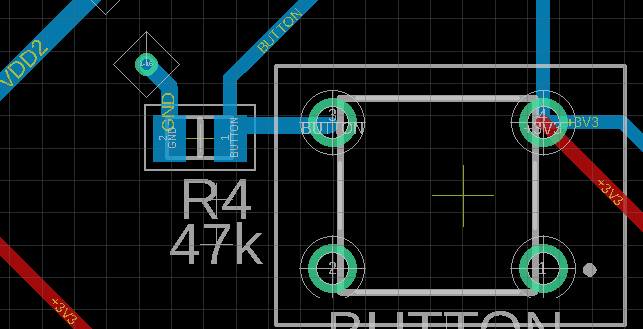
\includegraphics[width=0.8\textwidth]{figures/hardware/Via.PNG}
    \caption{How an SMD component on the bottom layer connects to the GND surface on the top layer}
    \label{fig:via}
\end{figure}

\FloatBarrier

\subsubsection{Design Rules Check (DRC)}

Once the traces are in place, a final check has to be performed, before the board is handed to the manufacturer. Luckily, Eagle provides a straight-forward tool to check for minimal distances between components and traces, overlapping, floating connections and other issues: The DRC (Design Rules Check).

In our case, the manufacturer PCB-Pool provides a set of their own rules about minimum trace width, via points, clearance rules etc. After incorporating it in Eagle and checking, all of the found issues need to be fixed, before the board is ready for production.
An instance of the interface can be seen in Fig. \ref{fig:drc}.

\begin{figure}[htb]
    \centering
    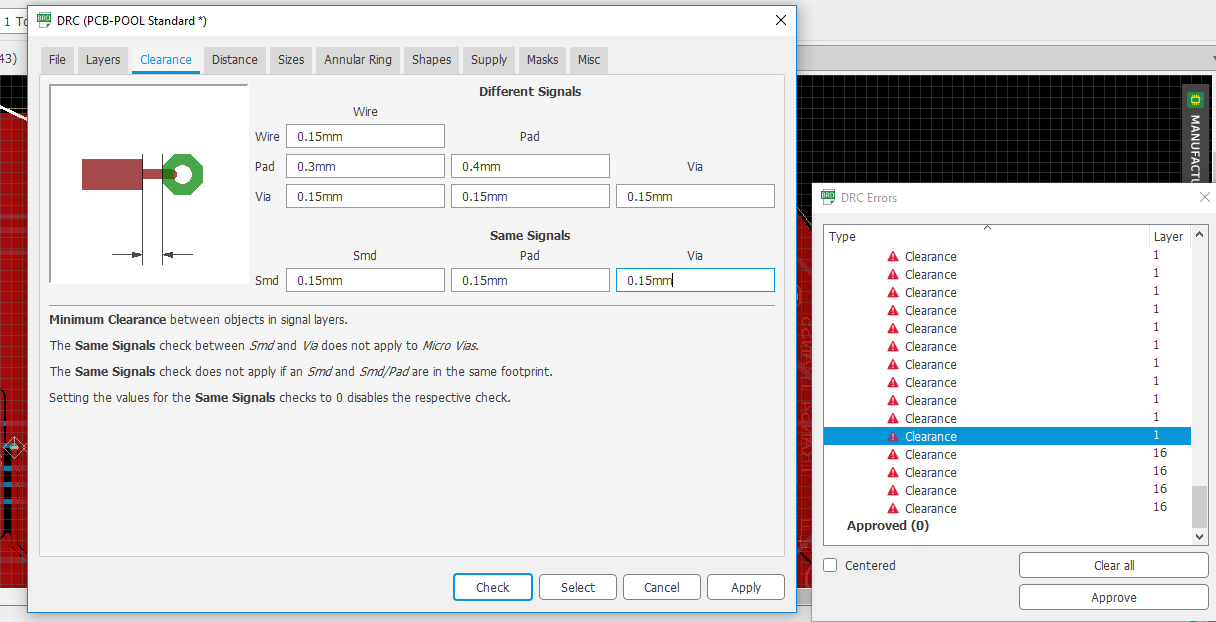
\includegraphics[width=1\textwidth]{figures/hardware/DRC.PNG}
    \caption{Interface of DRC and list of found violations}
    \label{fig:drc}
\end{figure}


\FloatBarrier
\vspace{1cm}

\subsection{Casing}

To house not only the PCB, but also sensors ,motors and the battery in a safe and robust way, a set of casing for the micromouse is designed and 3D printed.

\begin{figure}[htb]
    \centering
    \begin{minipage}{.45\textwidth}
          \centering
            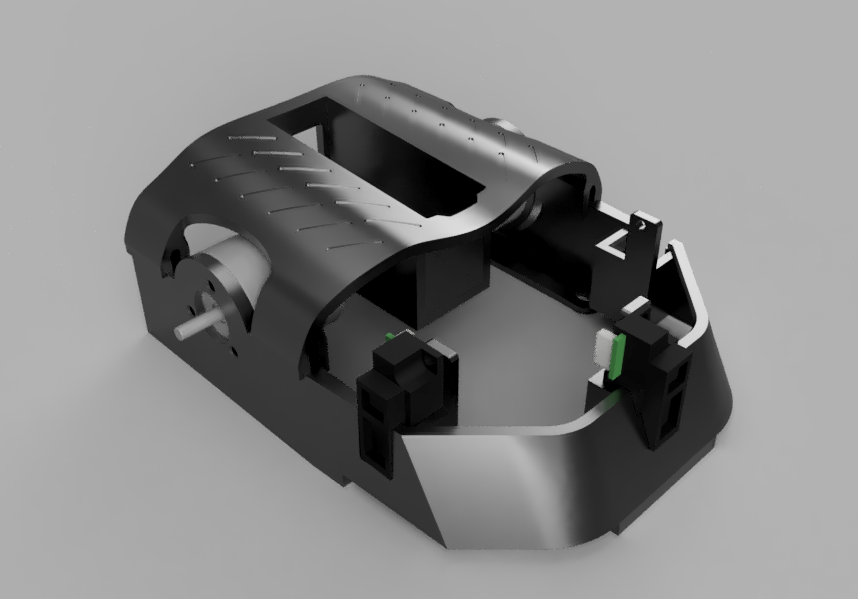
\includegraphics[width=.9\linewidth]{figures/Casing/CADrendering.png}
              \caption{A rendering of the MicroMouse casing CAD 3D Model}
    \end{minipage}
    \begin{minipage}{.45\textwidth}
          \centering
            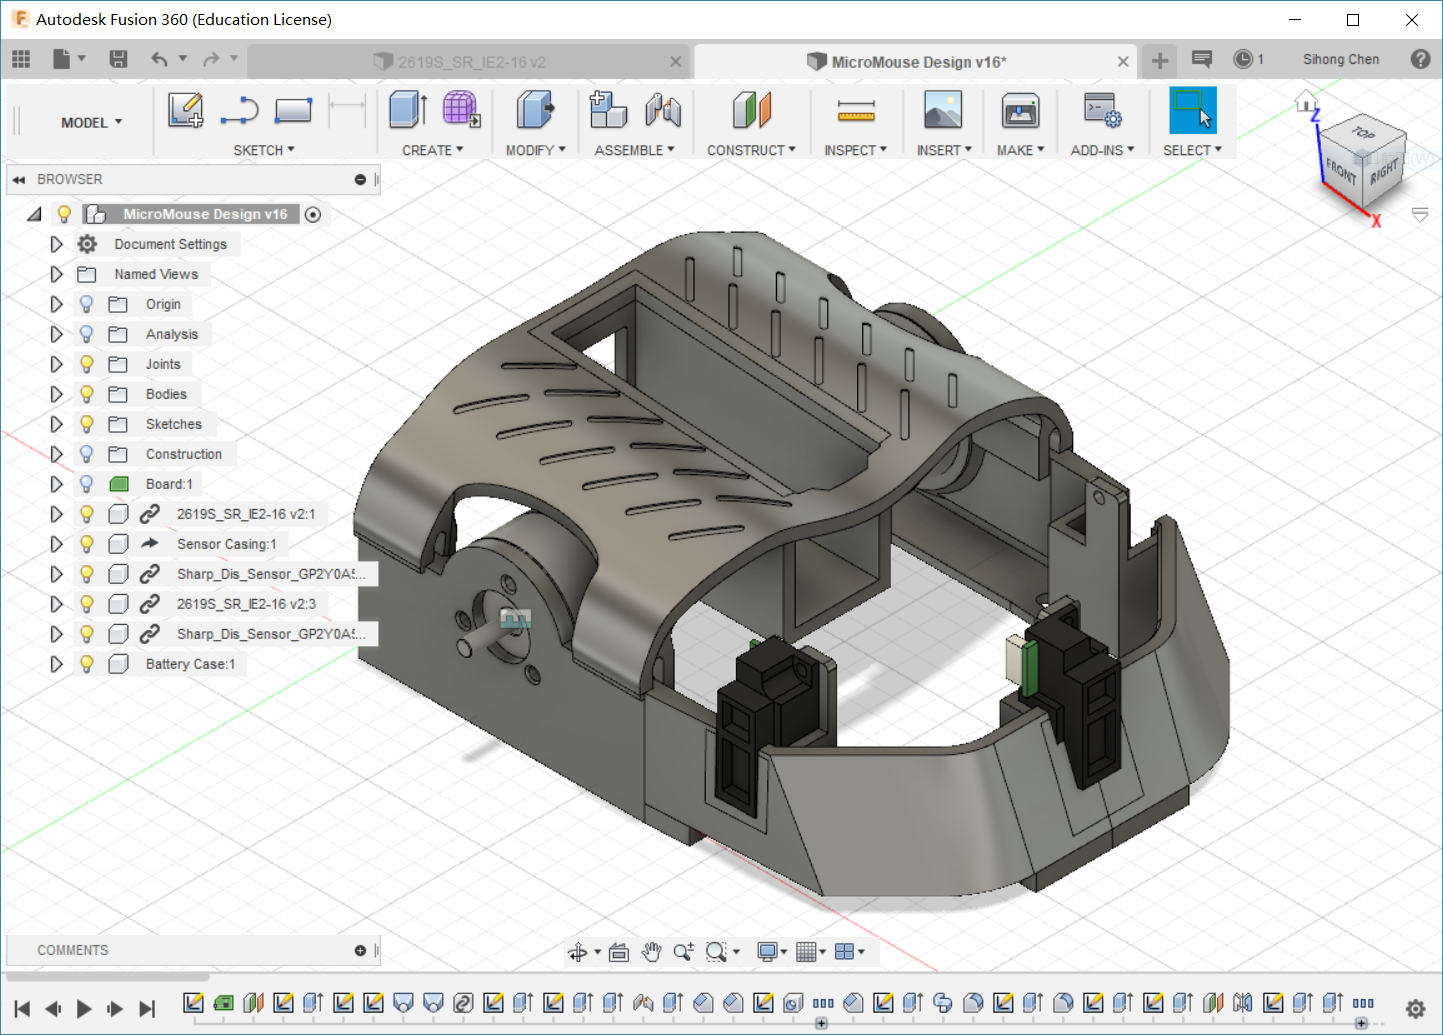
\includegraphics[width=.9\linewidth]{figures/Casing/FusionModelling.PNG}
              \caption{MicroMouse casing in Fusion 360 CAD modelling environment}
                \label{fig:CaseModelling}
    \end{minipage}
\end{figure}

\subsubsection{CAD Modelling}
\begin{itemize}
    \item Base Casing\\ 
    This casing is the encompassing platform, on which all hardware components are placed. See figure \ref{fig:CaseModelling} for the CAD model of the base casing.

    PCB rests on the bottom wrapper, and is fastened on with screws. Motors are mounted on the side with screws as well. Sensors are placed one front centre, another two facing left and right.

    In this CAD model, there are several components. Other than the base wall, the most prominent components are the sensor casings. These are actually one component, but imported on three positions, modified according to other components and integrated into the assembly design. 

    The approach to model the sensor casing separately as a component and later integrate reduces duplicate work. This separation also ensures that even a change in sensor model would only result in limited modification work to the final design.
    

    \item Battery Cover\\ 
    In order to secure the battery safely and make our robot space efficient, a battery cover is designed to hold the battery above PCB and other components. It also serves as a covering case for aesthetic purposes to some extent.

    This cover is designed to be a snap fit with the base casing, see figure \ref{fig:SnapFitBase} and \ref{fig:SnapFitCover}.

    For designing the surface of this cover, the free-form modelling and sculpting feature is used, in addition to the more traditional parametric modelling and solid modelling. This allows us to more easily model a visually pleasing surface to the design, giving our mouse a more “sporty” look, rather than the usual “boxy” appearance from more traditional CAD methods.

    In the design of the battery cover, attention was paid to reduce overhanging structure, so that the supporting structures needed are minimised. For example, the front side of the battery holder is left empty, as it eliminates support structure when this part is printed vertically (front is facing up). However, some support is unavoidable, for example when there is enclosing structure such as a circle.

\end{itemize}

\begin{figure}[htb]
    \centering
    \begin{minipage}{.45\textwidth}
          \centering
            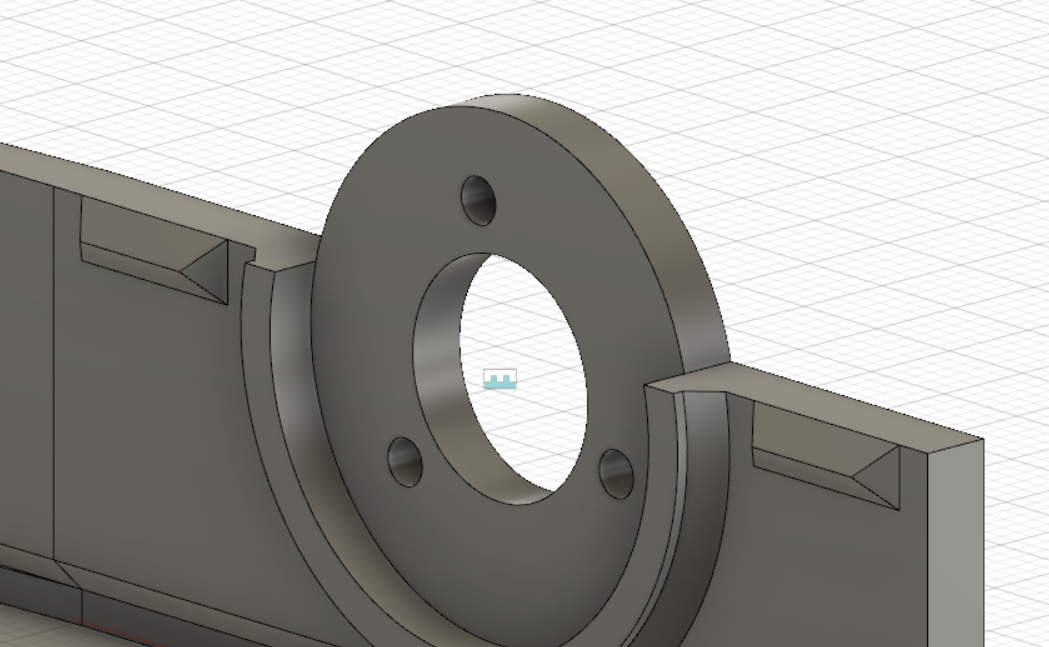
\includegraphics[width=.9\linewidth]{figures/Casing/SnapFitBase.PNG}
              \caption{Snap fit design on the base part}
                \label{fig:SnapFitBase}
    \end{minipage}
    \begin{minipage}{.45\textwidth}
          \centering
            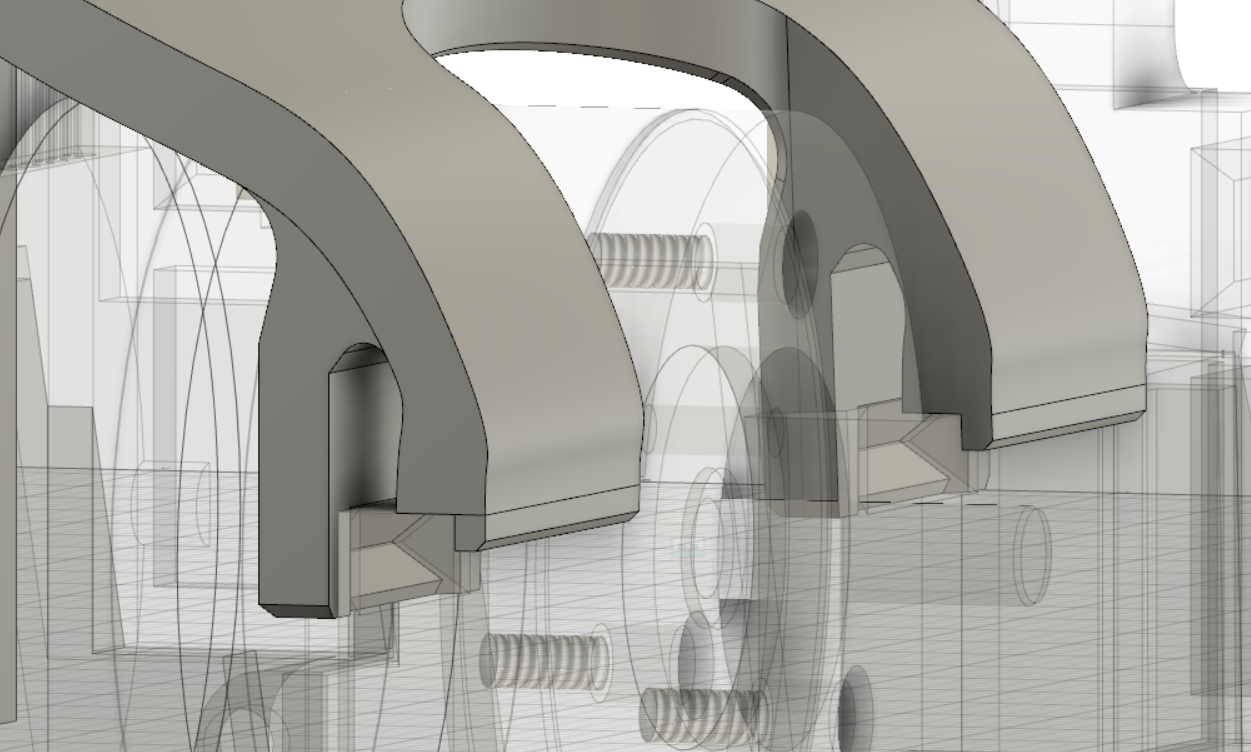
\includegraphics[width=.9\linewidth]{figures/Casing/SnapFitCover.PNG}
              \caption{Snap fit design on the cover part}
                \label{fig:SnapFitCover}
    \end{minipage}
\end{figure}

\subsubsection{3D printing the casing}
\begin{itemize}
    \item Method\\ 
    There are many types of 3D printing process, most common ones include Material Extrusion method such as Fused Deposition Modeling (FDM), and Vat Polymerization such as Stereolithography (SLA), Direct Light Processing (DLP). FDM is most widely available method of 3D printing, meanwhile SLA has a better dimensional accuracy (lower limit $\pm$ 0.10 mm in a desktop SLA printer compared to lower limit $\pm$ 0.5 mm in a desktop FDM printer).

    The 3D printing method we used is Fused Deposition Modeling (FDM). Out of the two available 3D printer FDM and SLA, the FDM method is chosen for its shorter lead and print time, as it does not require a curing process as for SLA. The dimensional accuracy is also acceptable to our application.
    
\begin{figure}[htb]
    \centering
    \begin{minipage}{.45\textwidth}
          \centering
            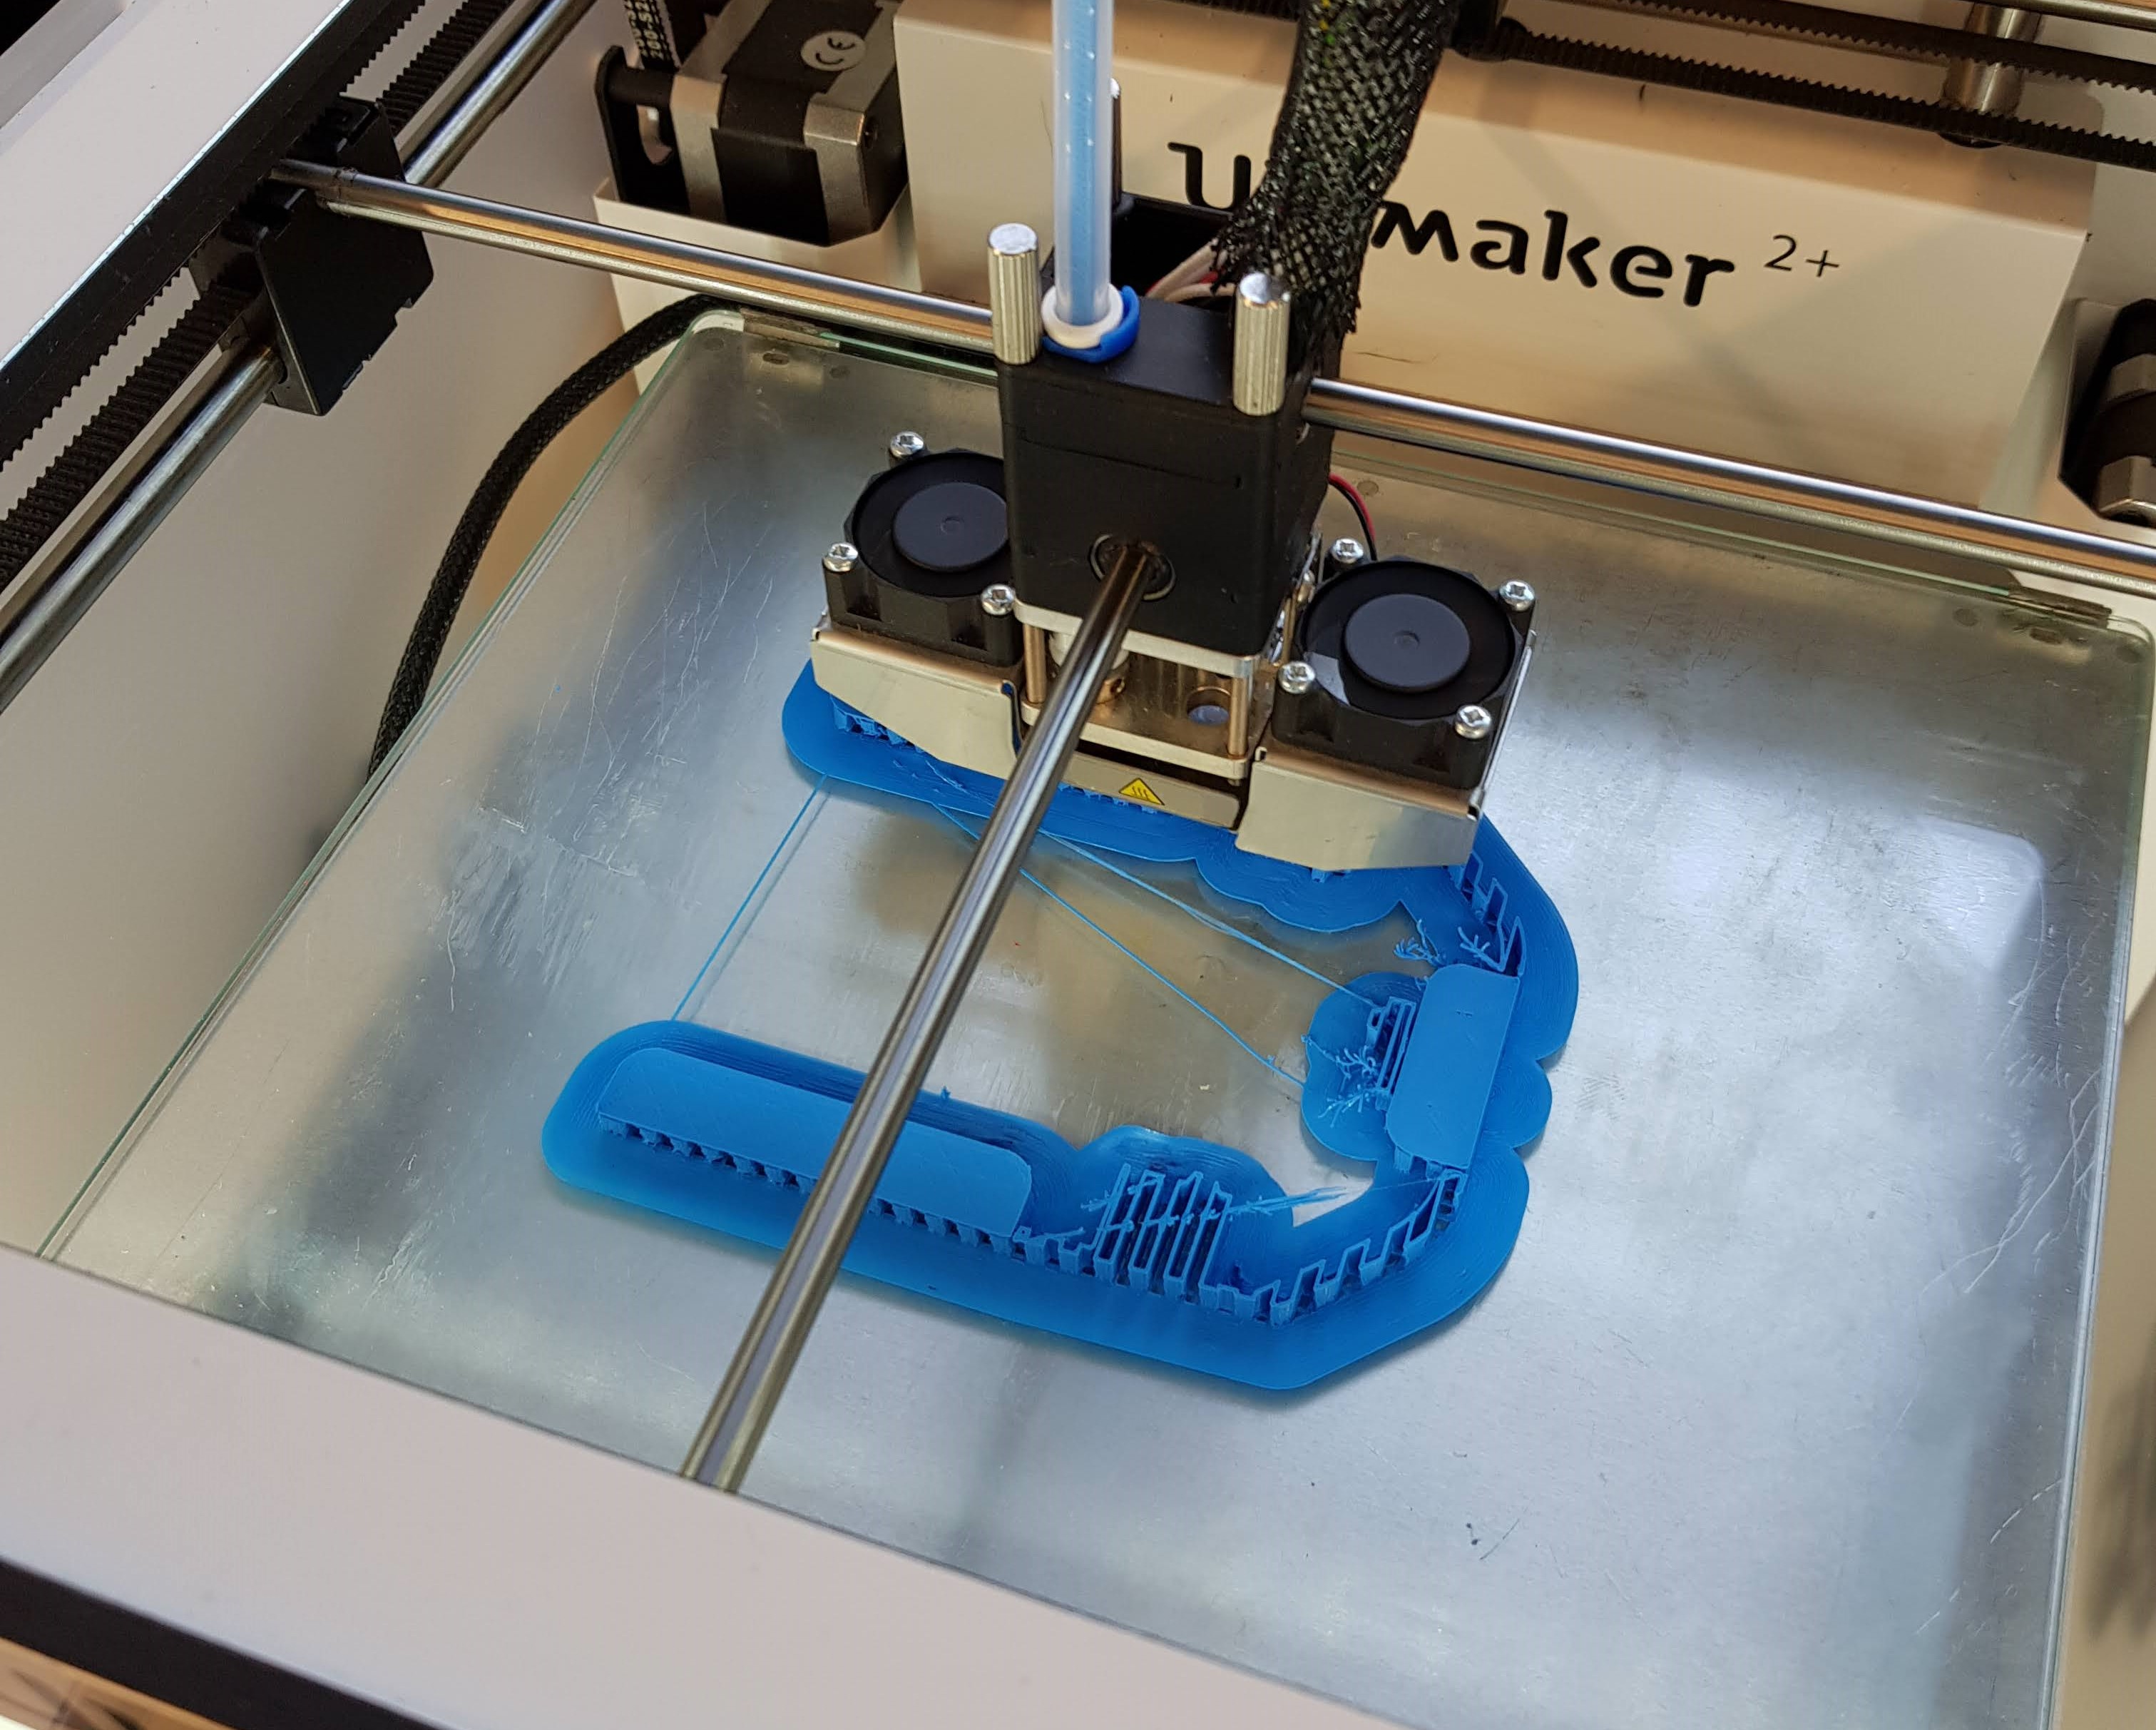
\includegraphics[width=.9\linewidth]{figures/Casing/PrintingProcess.jpg}
              \caption{A Case being printed}
    \end{minipage}
    \begin{minipage}{.45\textwidth}
          \centering
            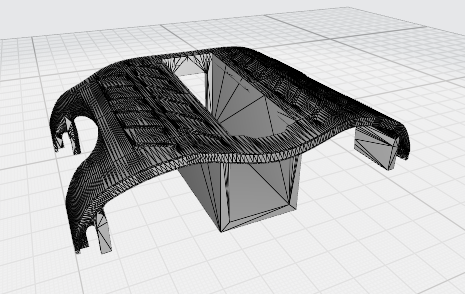
\includegraphics[width=.9\linewidth]{figures/Casing/Battery_Case_Micromouse_STL.png}
              \caption{Model in STL format for slicer program to process}
    \end{minipage}
\end{figure}
    
    \item Material\\ 
    There are two kinds of material for the FDM printer available for us, which are also the two most widely used materials for FDM 3D printing, namely PLA (Polylactic Acid) and ABS (Acrylonitrile Butadiene Styrene). They both can be used to print dimensional accurate parts, with very similar cost. PLA is under correct condition biodegradable, whereas ABS is not but recyclable.

    ABS is chosen for our project due to its improved ductility, higher flexural strength, and slightly better mechanical properties. Because ABS is less brittle than PLA, it has also better machinability, that means drilling hole or sanding would be easier, which we will likely do, whereas PLA would require more care during such post-processing.

    \item Process\\ 
    For this project, the 3D print process includes generating STL file from 3D CAD model, slicing and adding support structure, printing, and post processing work.

    One problem that often occurs during 3D printing is handling critical surface, therefore attention is paid to ensure that the critical surfaces in our design such as inside surface of sensor casing are all parallel or vertical to the platform plane, so that the 3D printer can produce a more precise and smooth result.

    Specialised programs or Slicers "cut" CAD models into layers and computes how the printer's extruder would assemble each layer. When necessary, support structures are also added in this stage, depending on if there is overhanging structures in the model.

    Post processing is mostly removing support structures from the printed parts, and sanding and polishing rough edges and surfaces.
\end{itemize}

\FloatBarrier
\vspace{1cm}

